\documentclass[sigplan,protrusion=true,expansion,screen]{acmart}

%\setlength{\belowcaptionskip}{-10pt}

\usepackage[utf8]{inputenc}
\usepackage[T1]{fontenc}
\usepackage{etoolbox}
\usepackage{mathtools}
\usepackage{thmtools}
\usepackage{empheq}
\usepackage{xspace}

% Diagrams.
\usepackage{tikz}
\usetikzlibrary{
  arrows,
  arrows.meta,
  calc,
  decorations.pathreplacing,
  decorations.text,
  math,
  positioning,
  shapes,
}

% Proof trees.
\usepackage{bussproofs}
\def\labelSpacing{0em}
\def\ScoreOverhang{0em}

\usepackage{stackengine}        % for breaking long lines in proof trees
\strutshortanchors{F}
\def\stackalignment{l}

% Enumerations.
\usepackage[inline]{enumitem}
\newlist{enumerate:a}{enumerate}{4}
\setlist[enumerate:a]{label=(\alph*)}
\newlist{enumerate:i}{enumerate}{4}
\setlist[enumerate:i]{label=(\roman*)}

% Proof by cases.
\newlist{case}{enumerate}{4}
\SetLabelAlign{case}{\emph{Case}~#1.\hfil}
\setlist[case]{itemsep=1ex,leftmargin=\parindent,labelindent=\parindent,
labelwidth=*,align=case,label*=.\arabic*}
\setlist[case,1]{label=\arabic*,leftmargin=0pt,labelindent=0pt}

% Values for \jot.
\newlength{\savedjot}
\setlength{\savedjot}{\jot}
\newlength{\rulejot}
\setlength{\rulejot}{2\savedjot}

% Notes
\usepackage[textsize=footnotesize]{todonotes}
\newcommand{\rc}[1]{\todo[inline,color=green!40]{\textbf{Rodrigo}: #1}}
\newcommand{\fs}[1]{\todo[inline,color=blue!40]{\textbf{Francisco}: #1}}
\newcommand{\gl}[1]{\todo[inline,color=red!40]{\textbf{Guilherme}: #1}}

% Céu.
\newcommand*{\CEU}{\textsc{C\'{e}u}\xspace}

% Full Céu.
\usepackage{listings}
\lstdefinelanguage{ceu}{%
  language=C,
  morekeywords={%
    @const, @pure, @safe, CHAN, FOREVER, PAR, PROC, SIGNAL, abort, and,
    await, bool, call, class, data, define, deterministic, do, each, else,
    emit, end, escape, event, every, finalize, hor, implementation, in,
    input, interface, loop, min, native, new, nohold, not, or, output, par,
    pool, pure, return, s, signal, spawn, tag, then, this, traverse, until,
    var, watching, when, with},
}
\lstset{
  showlines=true,
  basicstyle=\ttfamily,
  captionpos=b,
  columns=flexible,
  commentstyle=\rmfamily\itshape,
  escapeinside={||},
  frame=tb,
  keepspaces=true,
  keywordstyle=\bfseries,
  language=ceu,
  mathescape=true,
  numbersep=4pt,
  numberstyle=\scriptsize,
  upquote=true,
}
\newcommand{\code}[1]{{\relax{\footnotesize\texttt{#1}}}}
%\let\code\lstinline

% Basic Céu.
\makeatletter
\def\@int{\mathit{int}}
\def\@ext{\mathit{ext}}
\let\ext\@ext
\def\@ceuop#1{\mathop{\relax{\texttt{#1}}}}%
\def\@ceubin#1{\mathbin{\relax{\texttt{#1}}}}%
\def\ceu{\protect\@ceu}
\def\@ceu#1{%
  \bgroup
  \def\Block{\@ceuop{block}}%
  \def\Var{\@ceuop{var}}%
  \def\Id{\mathit{id}}%
  \def\Mem{\@ceuop{mem}}%
  \def\AwaitExt{\@ceuop{await}\nolimits_\@ext}%
  \def\AwaitInt{\@ceuop{await}\nolimits_\@int}%
  \def\EmitInt{\@ceuop{emit}\nolimits_\@int}%
  \def\Break{\@ceuop{break}}%
  \def\IfElse##1##2##3{\@ceuop{if}##1\@ceuop{then}{##2}\@ceuop{else}{##3}}%
  \def\Loop{\@ceuop{loop}}%
  \def\Every{\@ceuop{every}}%
  \def\And{\@ceubin{and}}%          to be removed
  \def\Or{\@ceubin{or}}%            to be removed
  \def\ParAnd{\@ceubin{par/and}}%
  \def\ParOr{\@ceubin{par/or}}%
  \def\Fin{\@ceuop{fin}}%
  \def\Nop{\@ceuop{@nop}}%
  \def\CanRun{\@ceuop{@canrun}}%    to be removed
  \def\RunAt{\@ceuop{@runat}}%
  \def\Restore{\@ceuop{@restore}}%
  \def\AtLoop{\@ceuop{@loop}}%
  \def\AtAnd{\@ceubin{@and}}%       to be removed
  \def\AtOr{\@ceubin{@or}}%         to be removed
  \def\AtParAnd{\@ceubin{@par/and}}%
  \def\AtParOr{\@ceubin{@par/or}}%
  \ensuremath{#1}\ignorespaces
  \egroup
}
\makeatother

% Math.
\def\<#1>{\langle#1\rangle}
\let\nil\varepsilon
\newcommand*{\doubleplus}{\mathbin{+\mkern-7mu+}}

% Metavariables.
\newcommand*\expr{\mathit{expr}}
\newcommand*\stmt{\mathit{stmt}}
\newcommand*\vars{\mathit{vars}}

% Functions.
\newcommand*\memdecl{\mathop{\mathit{decl}}}
\newcommand*\memeval{\mathop{\mathit{eval}}}
\newcommand*\memrest{\mathop{\mathit{rest}}}
\newcommand*\memupdt{\mathop{\mathit{updt}}}
\newcommand*\reaction{\mathop{\mathit{reaction}}}

% Proof environments: assumptions and proof-by-cases.
\makeatletter
\AtEndPreamble{%
  \theoremstyle{definition}
  \newtheorem{assumption}[theorem]{Assumption}}
\makeatother

% Functions bcast, clear, eval, and isblocked.
\makeatletter
\let\op\operatorname
\newcommand{\opi}[1]{\op{\mathit{#1}}}
%%
\def\eval{\opi{eval}}
\def\bcast{\opi{bcast}}
\def\clear{\opi{clear}}
\def\isblockedext{\opi{isblocked}_\@ext}
\def\isblocked{\opi{isblocked}}
\def\pot{\opi{pot}}
\def\rank{\opi{rank}}
\makeatother

% Rule labels.
\makeatletter
\def\@R#1{{\bfseries#1}}
\def\Rtag#1{\tag{\@R{#1}}\label{R:#1}}
\def\R#1{\hyperref[R:#1]{\@R{#1}}}
\makeatother

% Transition arrows.
\makeatletter
\newcommand{\@trans}[2][]{%
  \setbox0=\hbox{$\mathord{\longrightarrow}$}%
  \mathbin{%
    \mathrlap{\longrightarrow}%
    \notblank{#2}{%
      \rlap{\raisebox{-3pt}%
        {\makebox[\wd0][c]{\ensuremath{\scriptstyle#2}}}}%
    }{}%
    \notblank{#1}{%
      \rlap{\raisebox{5pt}%
        {\makebox[\wd0][c]{\ensuremath{\scriptstyle#1}}}}%
    }{}%
    \phantom{\longrightarrow}%
  }%
}
\newcommand{\trans}[1][]{\@trans[#1]{}}
\newcommand{\@out}{\mathit{out}}
\newcommand{\@nst}{\mathit{nst}}
\newcommand{\out}[1][]{\@trans[#1]{\@out\,\;}}
\newcommand{\outpush}{\out[\mathit{push}]}
\newcommand{\outpop}{\out[\mathit{pop}]}
\newcommand{\nst}[1][]{\@trans[#1]{\@nst\,\;}}
\makeatother

% Irreducible predicate.
\makeatletter
\newcommand{\Hout}{{\#\@out}}
\newcommand{\Hnst}{{\#\@nst}}
\makeatother

% Hacks to reduce the space after captions.
\setlength{\textfloatsep}{.5\baselineskip}
\setlength{\intextsep}{.5\baselineskip}

%%% Local Variables:
%%% mode: latex
%%% TeX-master: "index.tex"
%%% End:

% Copyright
%\setcopyright{none}
%\setcopyright{acmcopyright}
%\setcopyright{acmlicensed}
%\setcopyright{rightsretained}
%\setcopyright{usgov}
%\setcopyright{usgovmixed}
%\setcopyright{cagov}
%\setcopyright{cagovmixed}

% DOI
%\acmDOI{10.475/123_4}

% ISBN
%\acmISBN{123-4567-24-567/08/06}

%Conference
%\acmConference[LCTES'18]{ACM SIGPLAN/SIGBED}{June 2018}{Philadelphia, USA}
%\acmYear{1997}
%\copyrightyear{2016}

%\acmPrice{15.00}

%\acmBadgeL[http://ctuning.org/ae/ppopp2016.html]{ae-logo}
%\acmBadgeR[http://ctuning.org/ae/ppopp2016.html]{ae-logo}

%%% If you see 'ACMUNKNOWN' in the 'setcopyright' statement below,
%%% please first submit your publishing-rights agreement with ACM (follow link on submission page).
%%% Then please update our instructions page and copy-and-paste the NEW commands into your article.
%%% Please contact us in case of questions; allow up to 10 min for the system to propagate the information.
%%%
%%% The following is specific to LCTES'18 and the paper
%%% 'A Memory-Bounded, Deterministic and Terminating Semantics for the Synchronous Programming Language Céu'
%%% by Guilherme F. Lima, Rodrigo C. M. Santos, Edward Hermann Haeusler, Roberto Ierusalimschy, and Francisco Sant'Anna.
%%%
%\setcopyright{ACMUNKNOWN}
\setcopyright{acmcopyright}
\acmPrice{15.00}
\acmDOI{10.1145/3211332.3211334}
\acmYear{2018}
\copyrightyear{2018}
\acmISBN{978-1-4503-5803-3/18/06}
\acmConference[LCTES'18]{19th ACM SIGPLAN/SIGBED Conference on Languages, Compilers, and Tools for Embedded Systems}{June 19--20, 2018}{Philadelphia, PA, USA}

\begin{document}

\title[A Memory-Bounded, Deterministic and Terminating Semantics for~\CEU]
{A Memory-Bounded, Deterministic and Terminating Semantics for the
       Synchronous Programming Language~\CEU}

\author[Santos]{Rodrigo C.\,M.~Santos}
\affiliation{PUC-Rio, Brazil}
\email{rsantos@inf.puc-rio.br}
%
\author[Lima]{Guilherme F.~Lima}
\affiliation{PUC-Rio, Brazil}
\email{glima@inf.puc-rio.br}
%
\author[Sant'Anna]{Francisco Sant'Anna}
\affiliation{UERJ, Brazil}
\email{francisco@ime.uerj.br}
%
\author[Ierusalimschy]{Roberto Ierusalimschy}
\affiliation{PUC-Rio, Brazil}
\email{roberto@inf.puc-rio.br}
%
\author[Haeusler]{Edward H. Haeusler}
\affiliation{PUC-Rio, Brazil}
\email{hermann@inf.puc-rio.br}

\begin{abstract}
\CEU is a synchronous programming language for embedded soft real-time systems.
%
It focuses on control-flow safety features, such as safe shared-memory
concurrency and safe abortion of lines of execution, while enforcing
memory-bounded, deterministic, and terminating reactions to the environment.
%
In this work, we present a small-step structural operational semantics for
\CEU and a proof that reactions have the properties enumerated above:
%
that for a given arbitrary timeline of input events, multiple executions of the
same program always react in bounded time and arrive at the same final finite
memory state.
%
%We also discuss some equivalence results and the relation between the proposed
%semantics and its actual implementation.
\end{abstract}

\terms{Languages, design, theory}
\keywords{Determinism, Termination, Operational semantics, Synchronous languages}

\begin{CCSXML}
<ccs2012>
 <concept>
  <concept_id>10003752.10010124.10010131.10010134</concept_id>
  <concept_desc>Theory of computation~Operational semantics</concept_desc>
  <concept_significance>500</concept_significance>
 </concept>
 <concept>
  <concept_id>10011007.10011006.10011008.10011009.10011014</concept_id>
  <concept_desc>Software and its
                engineering~Concurrent programming languages</concept_desc>
  <concept_significance>500</concept_significance>
 </concept>
 <concept>
  <concept_id>10010520.10010553.10010562.10010564</concept_id>
  <concept_desc>Computer systems
                organization~Embedded software</concept_desc>
  <concept_significance>300</concept_significance>
 </concept>
</ccs2012>
\end{CCSXML}
\ccsdesc[500]{Theory of computation~Operational semantics}
\ccsdesc[500]{Software and its engineering~Concurrent programming languages}
\ccsdesc[300]{Computer systems organization~Embedded software}

\maketitle

\section{Introduction}
\label{sec.intro}

\CEU~\cite{ceu.sensys13,ceu.tecs17} is a Esterel-based~\cite{esterel.ieee91}
programming language for embedded soft real-time systems that aims to offer a
concurrent, safe, and expressive alternative to C with the characteristics that
follow:
%
\begin{description}
\item [Reactive:] code only executes in reactions to events.
\item [Structured:] programs use structured control mechanisms, such as
    \code{await} (to suspend a line of execution), and \code{par} (to combine
    multiple lines of execution).
\item [Synchronous:] reactions run atomically and to completion on each line of
    execution, i.e., there's no implicit preemption or real parallelism.
\end{description}
%
Structured reactive programming lets developers write code in direct style,
recovering from the inversion of control imposed by event-driven
execution~\cite{rp.deprecating,rp.rescala,sync_async.cooperative}.
%
Synchronous languages offer a simple run-to-completion execution model that
enables deterministic execution and make formal reasoning tractable.
For this reason, it has been successfully adopted in safety-critical real-time
embedded systems~\cite{rp.twelve}.

Previous work in the context of embedded sensor networks evaluates the
expressiveness of \CEU in comparison to event-driven code in C and attests a
reduction in source code size (around 25\%) with a small increase in memory
usage (around 5--10\%)~\cite{ceu.sensys13}.
%
\CEU has also been used in the context of multimedia
systems~\cite{ceumedia.webmedia16} and games~\cite{ceu.mod15}.
%, and as an
%alternative language in an undergraduate-level course on embedded systems for
%the past 6 years.

\CEU inherits the synchronous and imperative mindset of Esterel but adopts a
simpler semantics with fine-grained execution control.
%
The list that follows summarizes the semantic peculiarities of
\CEU~\cite{ceu.tecs17}:
%
\begin{itemize}
    \item Fine-grained, intra-reaction deterministic execution, which makes
          \CEU fully deterministic.
    \item Stack-based execution for internal events, which provides a limited
          but memory-bounded form of subroutines.
    \item Finalization mechanism for lines of execution, which makes abortion
          safe with regard to external resources.
    \item First-class timers with dedicated syntax, which provides automatic
          synchronization for multiple timers running simultaneously.
\end{itemize}

In this work, we present a formal small-step structural operational
semantics for \CEU and prove that it enforces memory-bounded, deterministic,
and terminating reactions to the environment, i.e., that for a given
arbitrary timeline of input events, multiple executions of the same program
always react in bounded time and arrive at the same final finite memory
state.
%
Conceiving a formal semantics for \CEU leads to a number of capabilities and
outcomes as follows:

\begin{enumerate}
\item
    Understanding, finding corner cases, and stabilizing the language.
    After the semantics was complete and discussed in extent in our group, we
    found a critical bug in the order of execution of statements.
\item
    Explaining core aspects of the language in a reduced, precise, and
    unambiguous way.
    This is particularly important when comparing languages that are similar in
    the surface (e.g., \CEU and Esterel).
\item
    Implementing the language.
    A small-step operational semantics describes an abstract machine that is
    close to a concrete implementation.
    The current implementation of the \CEU scheduler is based on the formal
    semantics presented in this paper.
\item
    Proving properties for particular or all programs in the language.
    For instance, in this work, we prove that all programs in \CEU are memory
    bounded, deterministic, and react in finite time.
\end{enumerate}

The last item is particularly important in the context of constrained embedded
systems:

\begin{description}
\item[Memory Boundedness:]
At compile time, we can ensure that the program fits in the device's restricted
memory and that it will not grow unexpectedly during runtime.
\item[Deterministic Execution:]
We can simulate an entire program execution providing an input history with the
guarantee that it will always have the same behavior.
This can be done in negligible time in a controlled development environment
before deploying the application to the actual device (e.g., by multiple
developers in standard desktops).
\item[Terminating Reactions:]
Real-time applications must guarantee responses within specified deadlines.
A terminating semantics enforces upper bounds for all reactions and guarantees
that programs always progress with the time.
\end{description}

The rest of the paper is organized as follows:
%
Section~\ref{sec.ceu} is a review of the main characteristics of \CEU based on
previous work~\cite{ceu.sensys13,ceu.tecs17}, namely deterministic event-driven
execution, safe shared-memory concurrency, abortion and finalization for
concurrent lines of execution, and first-class synchronized timers.
%
Section~\ref{sec.sem} proposes a formal small-step operational semantics for
\CEU that encompasses all peculiarities of the language.
%
Section~\ref{sec.proofs} presents the proofs for the properties of memory
boundedness, deterministic execution, and terminating reactions, which apply
to all programs in \CEU.
%
Section~\ref{sec.related} compares the semantics of \CEU with related
synchronous languages.
%
Section~\ref{sec.conclusion} concludes the paper.

\section{\CEU}
\label{sec.ceu}

\CEU~\cite{ceu.sensys13,ceu.tecs17} is a synchronous reactive language in which
programs evolve in a sequence of discrete reactions to external events.
%
It is designed for control-intensive applications, supporting concurrent lines
of execution, known as \emph{trails}, and instantaneous broadcast communication
through events.
%
Computations within a reaction (such as expressions, assignments, and
system calls) are also instantaneous considering the synchronous
hypothesis~\cite{rp.hypothesis}.
%
%\CEU provides an \code{await} statement which is the only that actually
%``consumes'' time.
%
\CEU provides an \code{await} statement that blocks the current running trail
allowing the program to execute its other trails; when all trails are blocked,
the reaction terminates and control returns to the environment.

In \CEU, every execution path within loops must contain at least one
\code{await} statement to an external input
event~\cite{ceu.sensys13,esterel.primer}.
%
\gl{Não seria melhor já dizer que todo caminho deve conter um \emph{await}
  externo \textbf{ou um \emph{break}}?}\noindent
%
This restriction, which is statically checked by the compiler, ensures that
every reaction runs in bounded time, eventually terminating with all trails
blocked in \code{await} statements.
%
\CEU has an additional restriction, which it shares with Esterel and
synchronous languages in general~\cite{esterel.preemption}: computations that
take a non-negligible time to run (e.g., cryptography or image processing
algorithms) violate the zero-delay hypothesis, and thus cannot be directly
implemented.

Listing~\ref{lst.syntax} shows a compact reference of~\CEU.

\def\C#1{\rmfamily\itshape//~#1}
\def\CC#1#2{\hfill\makebox[#1][l]{\C{#2}}}
\def\T<#1>{\langle\mathit{#1}\rangle}
\bgroup
\begin{figure}
\begin{lstlisting}[
  basicstyle=\ttfamily\small,
  caption={The concrete syntax of \CEU.},
  label={lst.syntax},
]
|\C{Declarations}|
input $\T<type>$ $\T<id>$; |\CC{19.5em}{declares an external input event} |
event $\T<type>$ $\T<id>$; |\CC{19.5em}{declares an internal event}       |
var   $\T<type>$ $\T<id>$; |\CC{19.5em}{declares a variable}              |

|\C{Event handling}|
$\T<id>$ = await $\T<id>$; |\CC{19.5em}{awaits event and assigns the received value} |
emit $\T<id>$($\T<expr>$); |\CC{19.5em}{emits event passing a value} |

|\C{Control flow}|
$\T<stmt>$ ; $\T<stmt>$ | \CC{8em}{sequence}     |
if $\T<expr>$ then $\T<stmt>$ else $\T<stmt>$ end | \CC{8em}{conditional}  |
loop do $\T<stmt>$ end | \CC{8em}{repetition}   |
every $\T<id>$ in $\T<id>$ do $\T<stmt>$ end | \CC{8em}{event iteration}   |
finalize [$\T<stmt>$] with $\T<stmt>$ end | \CC{8em}{finalization} |

|\C{Logical parallelism}|
par/or  do $\!\T<stmt>\!$ with $\!\T<stmt>\!$ end |\CC{10.5em}{aborts if any side ends}      |
par/and do $\!\T<stmt>\!$ with $\!\T<stmt>\!$ end |\CC{10.5em}{terminates if all sides end} |

|\C{Assignment \& Integration with C}|
$\T<id>$ = $\T<expr>$; | \CC{19.5em}{assigns a value to a variable}              |
_$\T<id>$($\T<exprs>$) | \CC{19.5em}{calls a C function (id starts with `\_'\,)} |
\end{lstlisting}
\end{figure}
\egroup

Listing~\ref{lst.ceu} shows a complete example in \CEU that toggles a LED
whenever a radio packet is received, terminating on a button press always
with the LED off.
%
The program first declares the \code{BUTTON} and \code{RADIO\_RECV} as
input events (ln~1--2).
Then, it uses a \code{par/or} composition to run two activities in parallel:
a single-statement trail that waits for a button press before terminating
(ln~4), and an endless loop that toggles the LED on and off on radio receives
(ln~9--14).
The \code{finalize} clause (ln~6--8) ensures that, no matter how its enclosing
trail terminates, the LED will be unconditionally turned off~(ln~7).

The \code{par/or} composition, which stands for a \emph{parallel-or}, provides
an orthogonal abortion mechanism~\cite{esterel.preemption} in which its
composed trails do not know when and how they are aborted (i.e., abortion is
external to them).
%
%This is possible to do safely in synchronous languages due to the accurate
%control of concurrent activities, i.e., in between every reaction, the whole
%system is idle and consistent~\cite{esterel.preemption}.
%
The finalization mechanism extends orthogonal abortion to %also work with
activities that use stateful resources from the environment (such as files and
network handlers), as we discuss in Section~\ref{sec.ceu.fin}.
%

In \CEU, any identifier prefixed with an underscore (e.g., \code{\_led}) is
passed unchanged to the underlying~C compiler.
%
Therefore, access to~C is straightforward and syntactically traceable.
%
To ensure that programs operate under the synchronous hypothesis, the compiler
environment should only provide access to~C operations that can be assumed to
be instantaneous, such as non-blocking~I/O and simple data structure accessors.%
\footnote {
The actual implementation of \CEU supports a command-line option that accepts a
whitelist of library calls.
If a program tries to use a function not in the list, the compiler raises an
error.
}

\begin{lstlisting}[
  xleftmargin=1em,
  numbers=left,
  basicstyle=\ttfamily\small,
  float=h,
  caption={A \CEU program that toggles a LED on receive,
           terminating on a button always with the LED~off.},
  label={lst.ceu},
]
input void BUTTON;
input void RADIO_RECV;
par/or do
    await BUTTON;
with
    finalize with
        _led(0);
    end
    loop do
        _led(1);
        await RADIO_RECV;
        _led(0);
        await RADIO_RECV;
    end
end
\end{lstlisting}

\subsection{External and Internal Events}
\label{sec.ceu.evts}

\CEU defines time as a discrete sequence of reactions to unique external
input events received from the environment.
%
Each input event delimits a new logical unit of time that triggers an
associated reaction.
%
The life-cycle of a program in \CEU can be summarized as
follows~\cite{ceu.sensys13}:
%
\begin{enumerate:i}
\item The program initiates a ``boot reaction'' in a single trail (parallel
      constructs may create new trails).
\item Active trails execute until they await or terminate, one after
      another.  This step is called a \emph{reaction chain}, and always runs in
      bounded time.
\item When all trails are blocked, the program goes idle and the environment
      takes control.
\item On the occurrence of a new external input event, the environment
      awakes \emph{all} trails awaiting that event, and the program goes back to
      step~(ii).
\end{enumerate:i}

A program must react to an event completely before handling the next one.
%
By the synchronous hypothesis, the time the program spends in step~(ii) is
conceptually zero (in practice, negligible).
%
Hence, from the point of view of the environment, the program is always
idle on step~(iii).
%
In practice, if a new external input event occurs while a reaction executes,
the event is saved on a queue, which effectively schedules it to be processed
in a subsequent reaction.

\subsubsection{External Events and Discrete Time}

The sequential processing of external input events induces a discrete notion of
time in \CEU, as illustrated in Figure~\ref{fig.ticks}.
%
The continuous timeline shows an absolute reference clock with ``physical
timestamps'' for the event occurrences (e.g., event~\code{C} occurs at
17ms521us).
%
The discrete timeline shows how the same occurring events fit in the logical
notion of time of \CEU.
%
The boot reaction \code{boot-0} happens before any input, at program startup.
%
Event~\code{A} ``physically'' occurs during \code{boot-0} but, because time
is discrete, its corresponding reaction only executes afterwards, at logical
instant~\code{A-1}.
%
Similarly, event~\code{B} occurs during~\code{A-1} and its reaction is
postponed to execute at~\code{B-2}.
%
Event~\code{C} also occurs during~\code{A-1} but its reaction must also wait
for~\code{B-2} to execute and so it is postponed to execute at~\code{C-3}.
%
Finally, event~\code{D} occurs during an idle period and can start immediately
at \code{D-4}.
%
%Finally, two instances of event~\code{E} occur during~\code{D-4}; they are
%handled in the subsequent reactions~\code{E-5} and~\code{E-6}.

\begingroup
\begin{figure}[b!]
\centering
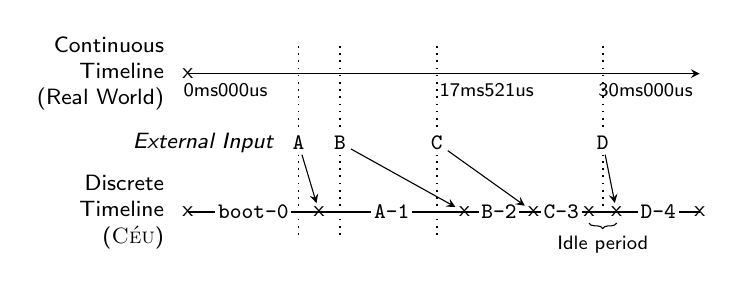
\begin{tikzpicture}[x=1em,y=1em,
  font=\footnotesize\sffamily,>=stealth,
  time/.style={font=\scriptsize\sffamily},
  cross/.style={inner sep=0pt,outer sep=0pt},
  evt/.style={fill=white,inner sep=1.85pt,outer sep=0pt},
  rng/.style={fill=white,inner sep=1pt,outer sep=0pt,
    font=\ttfamily\footnotesize}]
  \draw[->]
  (0,0)
    node[align=right,anchor=east,xshift=-.5em]
        {Continuous\\Timeline\\(Real World)}
    node[anchor=north west,xshift=-.5em,time]
        {0ms000us}
    node[anchor=north west,xshift=8.75em,time]
        {17ms521us}
  -- (18.5,0)
    node[anchor=north east,xshift=.1em,time]
        {30ms000us};
  \node[cross] at (0,0){x};
  %%
  \coordinate(Ext) at ($(0,0)!.5!(0,-5)$);
  \coordinate(A) at (Ext-|4,0);
  \coordinate(B) at (Ext-|5.5,0);
  \coordinate(C) at (Ext-|9,0);
  \coordinate(D) at (Ext-|15,0);
  %%
  \draw[semithick,dotted] (0,1-|A) -- (0,-6-|A);
  \draw[semithick,dotted] (0,1-|B) -- (0,-6-|B);
  \draw[semithick,dotted] (0,1-|C) -- (0,-6-|C);
  \draw[semithick,dotted] (0,1-|D) -- (0,-5-|D);
  \node[evt](Aevt) at (A) {\texttt{\textbf{A}}};
  \node[evt](Bevt) at (B) {\texttt{\textbf{B}}};
  \node[evt](Cevt) at (C) {\texttt{\textbf{C}}};
  \node[evt](Devt) at (D) {\texttt{\textbf{D}}};
  \node[anchor=east,xshift=-.5em] at (A){\emph{External Input}};
  %%
  \draw[-]
  (0,-5)
    node[align=right,anchor=east,xshift=-.5em]
        {Discrete\\Timeline\\(\CEU)}
  -- (18.5,-5);
  \node[cross](P0) at (0,-5){x};
  \node[cross](P1) at (4.75,-5){x};
  \node[cross](P2) at (10,-5){x};
  \node[cross](P3) at (12.5,-5){x};
  \node[cross](P4) at (14.5,-5){x};
  \node[cross](P5) at (15.5,-5){x};
  \node[cross](P6) at (18.5,-5){x};
  \node[rng] at ($(P0)!.5!(P1)$){boot-0};
  \node[rng] at ($(P1)!.5!(P2)$){A-1};
  \node[rng] at ($(P2)!.5!(P3)$){B-2};
  \node[rng] at ($(P3)!.5!(P4)$){C-3};
  \node[rng] at ($(P5)!.5!(P6)$){D-4};
  \draw[decorate,decoration={brace,raise=-1pt,mirror,amplitude=2pt}]
  ($(P4)+(0,-.5)$) -- node[below,time] {Idle period} ($(P5)+(0,-.5)$);
  %%
  \begin{scope}[shorten >=1.5pt]
  \draw[->] (Aevt) -- (P1);
  \draw[->] (Bevt) -- (P2);
  \draw[->] (Cevt) -- (P3);
  \draw[->] (Devt) -- (P5);
  \end{scope}
\end{tikzpicture}
\vskip-.6em
%\includegraphics[width=\columnwidth]{tick_min}
\caption{The discrete notion of time in \CEU.}
\label{fig.ticks}
\end{figure}
\endgroup

Unique input events imply mutually exclusive reactions, which execute
atomically and never overlap.
%
Automatic mutual exclusion is a prerequisite for deterministic reactions as
we discuss in Section~\ref{sec.sem}.
%
%8<- - - - - - - - - - - - - - - - - - - - - - - - - - - - - - - - - - - - -
% \gl{A não ser que seja desenvolvido (e.g., explicado e comparado com
%   Esterel) eu acho que o parágrafo anterior é dispensável.}
% \fs{Tirei o "simplifies resoning about concurrency".
%     O resto do parágrafo é absoluto e tenta dar a intuição das condições para
%     ter determinismo.}
%- - - - - - - - - - - - - - - - - - - - - - - - - - - - - - - - - - - - ->8

In practice, the synchronous hypothesis for \CEU holds if reactions execute
faster than the rate of incoming input events.
%
Otherwise, the program would continuously accumulate delays between physical
occurrences and actual reactions for the input events.
%
Considering the context of soft real-time systems,
%targeted by \CEU (e.g., sensor networks, multimedia systems, interactive games, etc.)
postponed reactions might be tolerated as long as they are infrequent and the
application does not take too long to catch up with real time.
%
Note that the synchronous semantics is also the norm in typical event-driven
systems, such as event dispatching in UI toolkits, game loops in game engines,
and clock ticks in embedded systems.

\subsubsection{Internal Events as Subroutines}

In \CEU, queue-based processing of events applies only to external input
events, i.e., events submitted to the program by the environment.
%
Internal events, which are events generated internally by the program via
\code{emit} statements, are processed in a stack-based manner.
%
Internal events provide a fine-grained execution control, and, because of their
stack-based processing, can be used to implement a limited form of subroutines,
as illustrated in Listing~\ref{lst.sub}.

In the example, the ``subroutine'' \code{inc} is defined as an event iterator
(ln~4--6) that continuously awaits its identifying event (ln~4), and
increments the value passed by reference (ln~5).
%
A trail in parallel (ln~8--11) invokes the subroutine through two consecutive
\code{emit} statements (ln~9--10).
%
Given the stack-based execution for internal events, as the first emit
executes, the calling trail pauses (ln~9), the subroutine awakes (ln~4), runs
its body (yielding \code{v=2}), iterates, and awaits the next ``call'' (ln~4,
again).
%
Only after this sequence does the calling trail resumes (ln~9), makes a new
invocation (ln~10), and passes the assertion test (ln~11).

\begin{lstlisting}[
  xleftmargin=1em,
  numbers=left,
  basicstyle=\ttfamily\small,
  float=h,
  caption={A ``subroutine'' that increments its argument.},
  label={lst.sub},
]
event int* inc;       |\C{declares subroutine "inc"}|
par/or do
    var int* p;
    every p in inc do |\C{implements "inc" as event iterator}|
        *p = *p + 1;
    end
with
    var int v = 1;
    emit inc(&v);     |\C{calls "inc"}|
    emit inc(&v);     |\C{calls "inc"}|
    _assert(v==3);    |\C{asserts result after the two returns}|
end
\end{lstlisting}
%\vskip-\baselineskip

%- multiple executions
%- footnote to distinguish from TECS

\CEU also supports nested \code{emit} invocations, e.g., the body of the
subroutine \code{inc} (ln~5) could \code{emit} an event targeting another
subroutine, creating a new level in the stack.
%
We can think of the stack as a record of the nested, fine-grained internal
reactions that happen inside the same outer reaction to a single external
event.

This form of subroutines has a significant limitation that it cannot express
recursion, since an \code{emit} to itself is always ignored as a running trail
cannot be waiting on itself.
%
That being said, it is this very limitation that brings important safety
properties to subroutines.
%
First, they are guaranteed to react in bounded time.
%
Second, memory for locals is also bounded, not requiring data stacks.

At first sight, the constructions ``\code{every e do $\T<\cdots>$ end}'' and
``\code{loop do await e; $\T<\cdots>$ end}'' seem to be equivalent.
However, the \code{loop} variation would not compile since it does not contain
an external input \code{await} (\code{e} is an internal event).
%
The \code{every} variation compiles because event iterators have an additional
syntactic restriction that they cannot contain \code{break} or \code{await}
statements.
%
This restriction guarantees that an iterator never terminates from itself and,
thus, always awaits its identifying event, essentially behaving as a safe
blocking point in the program.
%
For this reason, the restriction that execution paths within loops must
contain at least one external \code{await} is extended to alternatively contain
an \code{every} statement.
%
%
\gl{Verificar se a restrição do \emph{every} não conter \emph{breaks} ou
  \emph{awaits} está sendo tratada na semântica.  Verificar também a
  extensão da restrição dos \emph{loops} para o \emph{every}: todo caminho
  de execução dentro de loops deve conter um \emph{await} externo,
  \emph{break}, ou \emph{every}.  \textbf{Pergunta}: pode \emph{every}
  dentro de \emph{every}?}

\subsection{Shared-Memory Concurrency}
\label{sec.ceu.shared}

Embedded applications make extensive use of global memory and shared resources,
such as through memory-mapped registers and system calls to device drivers.
Hence, an important goal of \CEU is to ensure a reliable behavior for programs
with concurrent lines of execution sharing memory and interacting with the
environment.

In \CEU, when multiple trails are active in the same reaction, they are
scheduled in lexical order, i.e., in the order they appear in the program
source code.
%
For instance, consider the examples in Figure~\ref{lst.shared}, both
defining shared variables (ln~3), and assigning to them in parallel trails
(ln~6,9).

In Listing~\ref{lst.shared.a}, the two assignments to \code{x} can only execute
in reactions to different events \code{A} and \code{B} (ln~5,8), which cannot
occur simultaneously by definition.
Hence, for the sequence of events \code{A->B}, \code{x} becomes \code{4}
(\code{(1+1)*2}), while for \code{B->A}, \code{x} becomes \code{3}
(\code{(1*2)+1}).

In Listing~\ref{lst.shared.b}, the two assignments to \code{y} are simultaneous because
they execute in reaction to the same event \code{A}.
Since \CEU employs lexical order for intra-reaction statements, the execution
is still deterministic, and \code{y} always becomes \code{4} (\code{(1+1)*2}).
%
However, note that an apparently innocuous change in the order of trails
modifies the behavior of the program.
%
To mitigate this threat, \CEU performs concurrency checks at compile time to
detect conflicting accesses to shared variables:
if a variable is written in a trail segment, then a concurrent trail segment
cannot access that variable~\cite{ceu.sensys13}.
%
Nonetheless, the static checks are optional and are not a prerequisite for the
deterministic semantics of the language.

\begingroup
\begin{figure}[h!]
\begin{minipage}[t]{0.45\linewidth}
\begin{lstlisting}[
    numbers=right,
    basicstyle=\ttfamily\small,
    label={lst.shared.a},
    %caption={Accesses to \code{x} are never concurrent.},
    caption={\,},
]
input void A;
input void B;
var int x = 1;
par/and do
    await A;
    x = x + 1;
with
    await B;
    x = x * 2;
end
\end{lstlisting}
\end{minipage}%
%
\begin{minipage}[t]{0.53\linewidth}
%\begin{lstlisting}
\begin{lstlisting}[
    xleftmargin=1.75em,
    basicstyle=\ttfamily\small,
    label={lst.shared.b},
    %caption={Accesses to \code{y} are concurrent but still deterministic.},
    caption={\,},
]
input void A;
|\C{(empty line)}|
var int y = 1;
par/and do
    await A;
    y = y + 1;
with
    await A;
    y = y * 2;
end
\end{lstlisting}
\end{minipage}%
%\rule{8.4cm}{0.37pt}
\caption{Shared-memory concurrency in \CEU:
Listing~\ref{lst.shared.a} is never concurrent because the trails access
\code{x} atomically in different reactions;
Listing~\ref{lst.shared.b} is concurrent, but still deterministic, because both
trails access \code{y} atomically in the same reaction.}
\label{lst.shared}
\end{figure}
\endgroup

\subsection{Abortion and Finalization}
\label{sec.ceu.fin}

The \code{par/or} of \CEU is an orthogonal abortion mechanism because the two
sides in the composition need not be tweaked with synchronization primitives nor
state variables to affect each other.
%
In addition, abortion is \emph{immediate} in the sense that it executes
atomically inside the current micro reaction.
%
Immediate orthogonal abortion is a distinctive feature of synchronous languages
and cannot be expressed effectively in traditional (asynchronous)
multi-threaded languages~\cite{esterel.preemption,sync_async.threadsstop}.

However, aborting lines of execution that deal with resources may lead to
inconsistencies.
%
Therefore, \CEU provides a \code{finalize} construct to unconditionally
execute a series of statements even if the enclosing block is externally
aborted.

\CEU also enforces, at compile time, the use of \code{finalize} for system
calls that deal with pointers representing resources, as illustrated in the two
examples of Figure~\ref{lst.fin}.
%
%\begin{itemize}
 If \CEU \emph{passes} a pointer to a system call (Listing~\ref{lst.fin.a},
    ln~5), the pointer represents a \emph{local} resource (ln~2) that
    requires finalization (ln~7).
 If \CEU \emph{receives} a pointer from a system call return
    (Listing~\ref{lst.fin.b}, ln~4), the pointer represents an
    \emph{external} resource (ln~2) that requires finalization (ln~6).
%\end{itemize}

\CEU tracks the interaction of system calls with pointers and requires
finalization clauses to accompany them.
%
In Listing~\ref{lst.fin.a}, the local variable \code{msg}
(ln~2) is an internal resource passed as a pointer to \code{\_send} (ln~5),
which is an asynchronous call that transmits the buffer in the background.
If the block aborts (ln~11) before receiving an acknowledge from the
environment (ln~9), the local \code{msg} goes out of scope and the external
transmission now holds a \emph{dangling pointer}.
The finalization ensures that the transmission also aborts (ln~7).
%
In Listing~\ref{lst.fin.b}, the call to \code{\_fopen} (ln~4) returns an
external file resource as a pointer.
If the block aborts (ln~12) during the \code{await A} (ln~9), the file
remains open as a \emph{memory leak}.
The finalization ensures that the file closes properly (ln~6).
%
In both cases, the code does not compile without the \code{finalize}.%
\footnote{%
The compiler only forces the programmer to write the finalization clause, but
cannot check if it actually handles the resource properly.}

%\vspace{2cm}
\begin{figure}[h!]
\begin{minipage}[t]{0.46\linewidth}
\begin{lstlisting}[
    numbers=right,
    basicstyle=\ttfamily\small,
    label={lst.fin.a},
    caption={Local resource.},
]
par/or do
   var _msg_t msg;
   $\T<\cdots>$   |\C{prepare msg}|
   finalize
      _send(&msg);
   with
      _cancel(&msg);
   end
   await SEND_ACK;
with
   $\T<\cdots>$
end

\end{lstlisting}
\end{minipage}%
%
\begin{minipage}[t]{0.54\linewidth}
\begin{lstlisting}[
    xleftmargin=1.75em,
    basicstyle=\ttfamily\small,
    label={lst.fin.b},
    caption={External resource.},
]
par/or do
   var _FILE* f;
   finalize
      f = _fopen($\dots$);
   with
      _fclose(f);
   end
   _fwrite($\dots$, f);
   await A;
   _fwrite($\dots$, f);
with
   $\T<\cdots>$
end
\end{lstlisting}
\end{minipage}%
%\rule{8.4cm}{0.37pt}
\caption{%
\CEU enforces the use of finalization to prevent dangling pointers and memory leaks.}
\label{lst.fin}
\end{figure}

The finalization mechanism of \CEU is fundamental to preserve the orthogonality
of the \code{par/or} construct since the clean up code is encapsulated in the
aborted trail itself.

\subsection{ First-Class Timers }
\label{sec.ceu.timers}

Embedded systems typically rely on activities that react to
\emph{wall-clock time}%
\footnote{
By wall-clock time we mean the passage of time from the real world, measured in 
hours, minutes, etc.
}, such as timeout watchdogs and periodic sensor readings~\cite{esterel.delays}.
%
\CEU supports wall-clock timers through the \code{await}
statement~\cite{ceu.tecs17}, as illustrated in Listing~\ref{lst.timers}.
The \code{await} blocks the current running trail for the specified amount of
time (ln~2,4).

However, underlying system timers do not activate programs immediately with
zero delay due to intrinsic overhead, such as OS scheduling, interrupts with
higher priorities, or even losses due to clock resolutions.
%
We define the difference between a requested timeout and the actual expiring 
time as the \emph{residual delta time (delta)}.
Without explicit manipulation, the recurrent use of timed activities in a row 
(or in a loop) may accumulate a considerable amount of deltas that can lead to 
incorrect behavior in programs.

\CEU handles deltas automatically, as illustrated in Listing~\ref{lst.timers.a}.
Suppose that after the first \code{await~10ms} request (ln~2), the underlying
system gets busy and takes 15ms to notify \CEU.
%
The scheduler will notice that the \code{await} has not only already expired,
but is delayed with \code{delta=5ms}.
The awaiting trail awakes, sets \code{v=1} (ln~3), and then invokes
\code{await~1ms} (ln~4).
%
Notice that non-awaiting statements are considered to take no time in the
synchronous model (e.g, ln~3).
%
Since the current delta is still higher than the requested timeout
(i.e.~$5ms>1ms$), the trail is rescheduled for execution, now with
\code{delta=4ms}.

Delta compensation also makes timers in parallel to be perfectly synchronized.
%
In the example in Listing~\ref{lst.timers.b}, although the scheduler cannot
guarantee that the first trail terminates exactly in 11ms (ln~2,4), it can at
least ensure that it terminates before the second trail (yielding \code{v=1}),
because $10+1<12$.
%
A similar program in a language without first-class support for timers would 
depend on the execution timings for the code marked as \code{<...>} (ln~3),
making the reasoning about the execution behavior more difficult.

\begin{figure}[h!]
\begin{minipage}[t]{0.37\linewidth}
\begin{lstlisting}[
    numbers=right,
    basicstyle=\ttfamily\small,
    label={lst.timers.a},
    caption={Wall-clock await.},
]
var int v;
await 10ms;
v = 1;
await 1ms;
v = 2;




\end{lstlisting}
\end{minipage}
%
\begin{minipage}[t]{0.59\linewidth}
\begin{lstlisting}[
    xleftmargin=1.75em,
    basicstyle=\ttfamily\small,
    label={lst.timers.b},
    caption={Synchronized timers.},
]
par/or do
  await 10ms;
  <...> // non awaiting stmts
  await  1ms;
  v = 1;
with
  await 12ms;
  v = 2;
end
\end{lstlisting}
\end{minipage}
%\rule{8.5cm}{0.37pt}
\caption{ First-class timers in \CEU.
\label{lst.timers}
}
\end{figure}

%%% Local Variables:
%%% mode: latex
%%% TeX-master: "index.tex"
%%% End:

\def\JOT{.8\jot}

\section{Formal Semantics of~\CEU}
\label{sec.sem}

We now introduce and formalize the semantics of a reduced version of \CEU,
called \emph{basic \CEU}.  Although simpler than the full language presented
in Section~\ref{sec.ceu}, basic \CEU is expressive enough to capture all the
essential characteristics of full \CEU, in particular, the stack-based
execution policy for internal events.  Once basic \CEU is defined, the more
elaborate constructs of full \CEU can be easily defined on top of it, as we
shall see shortly.

The statements of basic \CEU are presented in Figure~\ref{fig.sem.syntax}.
In the figure, the metavariables~$v$, $e$, and~$n$ range over variable
identifiers, event identifiers, and integers.  The metavariable~$\vars$
denotes zero or more variable identifiers, and the metavariables~$\stmt$ and
$\expr$ denote statements and expressions.  For simplicity, we only consider
integer expressions; these are build up from integer constants and variables
by the usual mathematical operators ($+$, $-$, $\le$, \ldots).  We assume
that expression evaluation takes zero time and that it always produces an
integer value.  In places where a boolean value is expected, any nonzero
value means true while zero means false.

\begin{figure}[ht!]
\begingroup
\setlength{\jot}{0pt}
\begin{empheq}[box=\fbox]{alignat*=2}
  &\ceu{\Block{\vars\ \stmt}}&\quad&\text{\it declaration block}\\
  &\ceu{v\coloneqq\expr}    &&\text{\it assignment statement}\\
  &\ceu{\AwaitExt(e)}       &&\text{\it await external event}\\
  &\ceu{\AwaitInt(e)}       &&\text{\it await internal event}\\
  &\ceu{\EmitInt(e)}        &&\text{\it emit internal event}\\
  &\ceu{\Break}             &&\text{\it loop escape}\\
  &\ceu{\IfElse{\expr}{\stmt_1}{\stmt_2}}&&\text{\it conditional}\\
  &\ceu{\stmt_1\,;\,\stmt_2}&&\text{\it sequence}\\
  &\ceu{\Loop \stmt}        &&\text{\it infinite loop}\\
  &\ceu{\Every{e}\,\stmt}   &&\text{\it event iteration}\\
  &\ceu{\stmt_1\And\stmt_2} &&\text{\it par/and statement}\\
  &\ceu{\stmt_2\Or\stmt_2}  &&\text{\it par/or statement}\\
  &\ceu{\Fin\stmt}          &&\text{\it finalization statement}\\
  &\ceu{\Nop}               &&\text{\it dummy statement}\\
  &\ceu{\CanRun(n)}         &&\text{\it wait for stack level~$n$}\\
  &\ceu{\Restore(n)}        &&\text{\it restore environment}\\
  &\ceu{\stmt_1\AtLoop\stmt_2}&&\text{\it unwinded loop}\\
  &\ceu{\stmt_1\AtAnd\stmt_2}&&\text{\it unwinded par/and}\\
  &\ceu{\stmt_1\AtOr\stmt_2}&&\text{\it unwinded par/or}
\end{empheq}
\endgroup
\caption{The statements of basic \CEU.}
\label{fig.sem.syntax}
\end{figure}

We distinguish between three kinds of basic \CEU statements.  First, there
are those statements which are common in imperative languages, namely,
assignments, conditionals, sequences, loops, and breaks.  The~$\ceu{\Block}$
statement, which defines a block introducing local variables, is also a
statement of the first kind.  All of these common imperative statements
behave as usual and execute in zero time.

The statements of the second kind are those which are specific to \CEU.
These are the statements~$\ceu{\AwaitExt}$, $\ceu{\AwaitInt}$,
$\ceu{\EmitInt}$, and~$\ceu{\Every}$, which deal with events, the
statements~$\ceu{\And}$ and~$\ceu{\Or}$, which define parallel compositions,
and the statement~$\ceu{\Fin}$, which defines a finalization block.  These
basic \CEU statements are more or less equivalent to their counterparts in
full \CEU.  We defer a precise description of their behavior and of the of
the properties entailed by this behavior to Section~\ref{sec.sem.opsem}.

Finally, the statements of the third kind are the remaining statements,
namely, $\ceu{\Nop}$, $\ceu{\CanRun}$, $\ceu{\Restore}$, $\ceu{\AtLoop}$,
$\ceu{\AtAnd}$, and~$\ceu{\AtOr}$.  These are hidden statements used by the
interpreter to encode in the program's text information about its execution.
We will have more to say about these \texttt{@}-statements in
Section~\ref{sec.sem.opsem}.  Before that, however, we need to present the
syntactical restrictions of basic \CEU and discuss the mapping of full \CEU
programs into basic \CEU programs.

\subsection{Syntactic Restrictions of Basic \CEU}
\label{sec.sem.restrictions}

The syntax of basic \CEU shown in Figure~\ref{fig.sem.syntax} can be seen as
a schema for generating programs.  Not all programs generated by this schema
are valid though.  To be considered a valid basic \CEU program, the program
must also satisfy the following restrictions.
\begin{enumerate}
\item\label{sec.sem.restrictions.1} If a statement of the
  form~$\ceu{\Loop{\stmt}}$ occurs in the program, then all execution paths
  within~$\stmt$ must contain an occurrence of a matching $\ceu{\Break}$ or
  an~$\ceu{\AwaitExt}$ statement or an~$\ceu{\Every}$ statement.
\item\label{sec.sem.restrictions.2} If a statement of the
  form~$\ceu{\Every{e}\,{\stmt}}$ or~$\ceu{\Fin{\stmt}}$ occurs in the
  program, then~$\stmt$ must contain an occurrences of $\ceu{\Loop}$,
  $\ceu{\Break}$, $\ceu{\AwaitExt}$, $\ceu{\AwaitInt}$, $\ceu{\Every}$,
  or~$\ceu{\Fin}$.
\end{enumerate}

The purpose of the first restriction is to ensure that the program does not
contain an infinite loop with a body that runs in zero time.  The purpose of
the second restriction is to ensure that the statements~$\ceu{\Every}$
and~$\ceu{\Fin}$ function as a safe blocking points in the program whose
bodies run in zero time.  Both restrictions are also present in full \CEU,
as discussed in Section~\ref{sec.ceu}.

% The~$\ceu{\Mem(id)}$ primitive represents a read or write to the memory
% location identified by~$id$.\footnotemark\
% 
% As the challenging parts of \CEU reside on its control structures, we are
% not concerned here with a precise semantics for side effects, but only
% with their occurrences in programs.
% 
% The special notation $nop$ is used to represent an innocuous $mem$
% expression (it can be thought as a synonym for $mem(\epsilon)$, where
% $\epsilon$ is an unused identifier).
% 
% \footnotetext{Although the same symbol~$\ceu{\Id}$ is used in their
%   definition, $\ceu{\Mem}$, $\ceu{\AwaitExt}$, $\ceu{\AwaitInt}$
%   and~$\ceu{\EmitInt}$ do not share identifiers: any identifier is either a
%   variable, an external event, or an internal event.}

%\subsection{Concrete Language Mapping}
\subsection{From \CEU to Basic \CEU}
\label{sec.sem.concrete}

With the exception of \texttt{@}-statements, most statements of basic \CEU
are also present in full \CEU.  These shared statements, however, are not
exactly equivalent.  It is often the case that a statement of basic \CEU
(say~$\ceu{\AwaitInt}$) lacks some of the features of its full \CEU
counterpart (\code{await}).  Moreover, some statements of full \CEU, such as
\code{finalize}, are simply not present in basic \CEU.  If we are to use
basic \CEU as a basis for implementing full \CEU then these gaps need to be
filled.  In this section, we discuss the three main gaps between the two
languages.  We leave out of the discussion the \texttt{@}-statements of
basic \CEU, as these are not exposed to end users.

% \texttt{@}-statements of basic \CEU are not considered in

% Although the abstract syntax presented in Figure~\ref{fig.sem.syntax} is
% similar to the concrete language in Listing~\ref{lst.syntax}, there are
% some significant mismatches between \CEU and the formal semantics that
% require some clarification.

% Also note that the \texttt{@}-statements do not exist in the concrete
% language and are results of expansions in the transition rules to be
% presented in Section~\ref{sec.sem.opsem}.

\subsubsection{\code{await} and \code{emit}}

The \code{await} and \code{emit} primitives of full \CEU are slightly more
complex than those of basic \CEU: they support communication of values
between emits and awaits.

Figure~\ref{lst.await_emit} shows a translation that adds a variable to hold
the value being communicated.
%
The original full \CEU code in Listing~\ref{lst.await_emit.a} declares an
internal event \code{e} (ln~2) and has an \code{await} (ln~4) and an
\code{emit} (ln~10) that communicate the value~$1$ between the trails in
parallel.
%
The translation to basic \CEU in Listing~\ref{lst.await_emit.b} declares an
additional shared variable \code{e\_} (ln~1) to hold the emitted value
(ln~9) and which can be accessed by the awaking trail (ln~5).

External events require a similar translation, i.e., each event needs a
corresponding global variable shared between all awaiting trails.

\begin{figure}[ht!]
\begin{minipage}[t]{0.48\linewidth}
\begin{lstlisting}[
    numbers=right,
    basicstyle=\ttfamily\small,
    caption={\,},
    label={lst.await_emit.a},
]

event int e;
par/or do
  var int v = await e;

  <...>
with
  <...>

  emit e(1);
end
\end{lstlisting}
\end{minipage}
%
\begin{minipage}[t]{0.45\linewidth}
\begin{lstlisting}[
    xleftmargin=1.75em,
    basicstyle=\ttfamily\small,
    caption={\,},
    label={lst.await_emit.b},
]
var int e_;
event int e;
par/or do
  await e;
  var int v = e_;
  <...>
with
  <...>
  e_ = 1;
  emit e;
end
\end{lstlisting}
\end{minipage}
%
\caption{ Concrete-to-abstract translation for \code{await} and \code{emit}. }
\label{lst.await_emit}
\end{figure}

\subsubsection{First-class timers}

To add support for first-class timers to basic \CEU , we introduce a
\code{TIMER} input event, which notifies the passage of time, and two global
variables: \code{timer\_} which holds the elapsed time, and \code{delta\_}
which holds the residual time, initially set to 0.

Listing~\ref{lst.TIMER.b} shows the basic \CEU program resulting from the
translation of the two timers shown in Listing~\ref{lst.TIMER.a} (ln~1,11).
A timer first adds a (possibly) negative delta from the time it should await
(ln~1).  Then, it enters in a loop that awakes on every occurrence of
\code{TIMER} (ln~7) and decrements the time it should await (ln~8).  Each
iteration of the loop checks if the timer has expired (ln~3), and sets the
new delta, which may affect a timer in sequence.  The check happens before
the await because the timer may already start expired due to the residual
time.

\begin{figure}[!ht]
\begin{minipage}[t]{0.33\linewidth}
\begin{lstlisting}[
    numbers=right,
    basicstyle=\ttfamily\small,
    caption={\,},
    label={lst.TIMER.a},
]
await 10ms;









await 1ms;

\end{lstlisting}
\end{minipage}
%
\begin{minipage}[t]{0.63\linewidth}
\begin{lstlisting}[
    xleftmargin=1.75em,
    basicstyle=\ttfamily\small,
    caption={\,},
    label={lst.TIMER.b},
]
var int tot_ = 10000 + delta_;
loop do
    if tot_ <= 0 then
        delta_ = tot_;
        break;
    end
    await TIMER;
    tot_ = tot_ - timer_;
end

var int tot_ = 1000 + delta_;
<...> // same loop as above
\end{lstlisting}
\end{minipage}
\caption{ Concrete-to-abstract translation for timers. }
\label{lst.TIMER}
\end{figure}

\subsubsection{Finalization}

\begin{comment}
Finally, a ``\code{finalize $A$ with $B$ end; $C$}'' in the concrete
language is equivalent to ``\ceu{A;\;((\Fin{B})\ \Or\ C)}'' in the abstract
language.  In the concrete language, $A$ and~$C$ execute in sequence, and
the finalization code~$B$ is implicitly suspended waiting for~$C$
to terminate.  In the abstract language, ``$\ceu{\Fin B}$'' suspends forever
when reached (it is an awaiting statement that never awakes).  Hence, we
need an explicit \code{or} to execute~$C$ in parallel, whose termination
aborts ``$\ceu{\Fin B}$'', which finally causes~$B$ to execute (by the
semantic rules below).
\end{comment}

The biggest mismatch between full \CEU and basic \CEU is in their support
for finalization, i.e., between the statements \code{finalize} of full \CEU
and $\ceu{\Fin}$ of basic \CEU.
%
Listing~\ref{3.lst.fin.a} shows a full \CEU program containing an explicit
block (ln~1,8) that executes the statements in \code{<A>} (ln~3) immediately
followed by \code{<C>} (ln~7), and unconditionally executes \code{<B>}
(ln~5) when the block terminates or aborts.
%
The simulate this behavior in basic \CEU we need to perform the translation
shown in Listing~\ref{3.lst.fin.b}.  This basic \CEU code also executes
\code{<A>} (ln~1) immediately followed by \code{<C>} (ln~5).  The difference
is that the \code{fin <B>} statement (ln~3) blocks the pending statement
forever, which only awakes and executes when it is aborted.  The
\code{par/or} (ln~2--6) serves this purpose since it allows \code{<C>} to
execute immediately and aborts the \code{fin} when terminating.

\begin{figure}[ht!]
\begin{minipage}[t]{0.48\linewidth}
\begin{lstlisting}[
    numbers=right,
    basicstyle=\ttfamily\small,
    caption={\,},
    label={3.lst.fin.a},
]
do
    finalize
        <A>
    with
        <B>
    end
    <C>
end
\end{lstlisting}
\end{minipage}
%
\begin{minipage}[t]{0.45\linewidth}
\begin{lstlisting}[
    xleftmargin=1.75em,
    basicstyle=\ttfamily\small,
    caption={\,},
    label={3.lst.fin.b},
]
<A>
par/or do
    fin <B>
with
    <C>
end


\end{lstlisting}
\end{minipage}
%
\caption{Concrete-to-abstract translation for finalization. }
\label{3.lst.fin}
\end{figure}

\subsection{Operational Semantics}
\label{sec.sem.opsem}

The operational semantics is a mathematical model that describes how an
abstract \CEU\ programs reacts to a single external input event, i.e., how
starting from this input event the program advances its state until all its
trails are blocked waiting for a another input event.
%%
The formalism we use here is that of small-step operational
semantics~\cite{Plotkin-G-D-1981} in which the meaning of programs is
defined in terms of transitions of an abstract machine.  Each transition
transforms a triple consisting of a program~$p$, a stack level~$n$, and an
emitted event~$e$ into a possibly different triple, i.e.,
\[
  \<p,n,e>\trans\<p',n',e'>\,,
\]
where~$p,p'\in\P$ are abstract-language programs, $n,n'\in\N$ are non-negative
integers representing the current stack level, and~$e,e'\in\E\cup\{\nil\}$ are
the events emitted before and after the transition (both possibly being the
empty event~$\nil$).
%$\E$ is a set of primitive events.

We refer to the triples on the left-hand and right-hand sides of
symbol~$\trans$ as \emph{descriptions} (denoted~$\delta$).  The description
on the left of~$\trans$ is called the \emph{input description}, the one on
its right is called the \emph{output description}.

%-
% \begin{align*}
% p, p' &\in\P
%     && (program~as~described~in~Listing~\ref{lst.formal.syntax})
% \\
% n, n' &\in\N
%     && (current~stack~level)
% \\
% e, e' &\in\E \cup \{\epsilon\}
%     && (emitted~event,~possibly~none)
% \end{align*}
%-

At the beginning of a reaction to an input event~$id$, the input description
is initialized with stack level~0 ($n=0$) and with the externally emitted
event~$e=\ceu{\Id}$.  At the end of a reaction, after an arbitrary but
finite number of transitions, the last output description will block with a
possibly modified program~$p'$ at stack level~0 and no event
emitted\footnote{We write~$\trans[i]$ to mean~$i$ transitions in sequence,
  and we write~$\trans[*]$ to mean a finite (possibly zero) number of
  transitions in sequence.}:
\[
  \<p,0,e>\mathbin{\trans[*]}\<p',0,\nil>\,.
\]

We now proceed to give the rules for possible the transitions.  We
distinguish between two types of transitions:  \emph{outermost transitions}
$\out$ and \emph{nested transitions} $\nst$\,.

\subsubsection{Outermost Transitions}

The rules \R{push} and \R{pop} for~$\out$ transitions are non-recursive
definitions that apply to the program as a whole.  These are the only rules
that manipulate the stack level.
\begin{gather*}
  \AxiomC{$e\ne\nil$}
  \UnaryInfC{$\<p,n,e>\out\<\bcast(p,e),n+1,\nil>$}
  \DisplayProof
  \Rtag{push}\\[1.2\jot]
  %%
  \AxiomC{$n>0$}
  \AxiomC{$p=\ceu{\Nop} \vee p=\ceu{\Break} \vee \isblocked(p,n)$}
  \BinaryInfC{$\<p,n,\nil>\out\<p,n-1,\nil>$}
  \DisplayProof
  \Rtag{pop}
\end{gather*}

%-
% { \setlength{\jot}{20pt}
% \begin{eqnarray*}
% & \frac
%     { \DS e \neq \epsilon }
% %   -----------------------------------------------------------
%     { \DS \LL p,n,e \RR \OUT \LL bcast(p),n+1,\epsilon \RR }
%     & \textbf{(push)}   \\
% %%%
% & \frac
%     { \DS n>0, \2 ((p=@nop) \vee isblocked(n,p)) }
% %   -----------------------------------------------------------
%     { \DS \LL p,n,\epsilon \RR \OUT \LL p,n-1,\epsilon \RR }
%     & \textbf{(pop)}    \\
% %%%
% %& \LL p,0,\epsilon \RR \1\xrightarrow\1 \bot
%     %& \textbf{(end)}    %\\
% \end{eqnarray*}
% }
%-

Rule \R{push} can be applied whenever there is a nonempty event in the input
description,
and instantly broadcasts the event to the program, which means
    (i)~awaking any active $\ceu{\AwaitExt}$ or $\ceu{\AwaitInt}$ statements
    (see $\bcast$ in
        Figure~\ref{fig.bcast}),
    (ii)~creating a nested reaction by increasing the stack level, and, at the same time,
    (iii)~consuming the event ($e$ becomes~$\nil$).
%
Rule \R{push} is the only rule that matches an
emitted event and also immediately consumes it.

Rule \R{pop} decreases the stack level by one and can only be applied if the
program is blocked (see $\isblocked$
in Figure~\ref{fig.isblocked}) or terminated ($p=\ceu{\Nop}$ or $p=\ceu{\Break}$).
This condition ensures that an $\ceu{\EmitInt}$ only resumes after its internal
reaction completes and blocks in the current stack level.

At the beginning of a reaction, an external event is emitted, which
triggers rule \R{push}, immediately raising the stack level
to~1.
At the end of the reaction, the program will block or terminate and
successive applications of
rule~\R{pop} will lead to a description with this
same program at stack level~0.

\subsubsection{Nested Transitions}

The~$\nst$ rules are recursive definitions of the form
\[
\<p,n,\nil>\nst\<p',n,e>.
\]
%
%-
% \begin{align*}
% \LL p, n,\epsilon \RR &\NST
% \LL p',n,e        \RR
%     & \textbf{(rule-inner)}
% \end{align*}
%-
%
Nested transitions do not affect the stack level and never have an emitted
event as a precondition.  The distinction between~$\out$ and~$\nst$ prevents
rules \R{push} and \R{pop} from matching and, consequently, from
inadvertently modifying the current stack level before the nested reaction
is complete.

A complete reaction consists of a series of transitions% of the form
\begin{align*}
  \<p,0,e_\ext>\outpush\<p_1,1,\nil>
  \Big[\null\nst[*]\null\out\null\Big]\!\!\ast
  \null\nst[*]\null\outpop\<p',0,\nil>\,,
\end{align*}
%
%-
% \begin{align*}
% a) &\5\5
%     \LL p,0,ext \RR
%         \1\xrightarrow[out]{push}\1
%     \LL q,1,\epsilon \RR
% \\
% b) &\5\5 \1[ \1\xrightarrow[in]{*}\1
%     \LL r,i,e \RR
%         \1\xrightarrow[out]\1
%     \LL s,j,\epsilon \RR \1]*
% \\
% c) &\5\5 \1\xrightarrow[in]{*}\1
%     \LL t,k,\epsilon \RR
%         \1\xrightarrow[out]{pop}\1
%     \LL u,0,\epsilon \RR
% \end{align*}
%-
%
First, a~$\outpush$ starts a nested reaction at level~1.  Then, a series of
alternations between zero or more~$\nst$ transitions (nested reactions) and
a single~$\out$ transition (stack operation) takes place.  Finally, a
last~$\outpop$ transition decrements the stack level to~0 and terminates the
reaction.

The~$\nst$ rules for atoms are defined as follows:
\begingroup
\def\JOT{-.1\jot}
\begin{align*}
  \<\ceu{\Mem(\Id)},n,\nil>
  &\nst\<\ceu{\Nop},n,\nil>\Rtag{mem}\\[\JOT]
  %%
  \<\ceu{\EmitInt(\Id)},n,\nil>
  &\nst\<\ceu{\CanRun(n)},n,\ceu{\Id}>\Rtag{emit-int}\\[\JOT]
  %%
  \<\ceu{\CanRun(n)},n,\nil>
  &\nst\<\ceu{\Nop},n,\nil>\Rtag{can-run}
\end{align*}
\endgroup

%-
% { \setlength{\jot}{20pt}
% \begin{align*}
% \LL mem(id), n, \epsilon \RR &\NST
% \LL @nop, n, \epsilon \RR
%     & \textbf{(mem)}        \\
% %%%
% \LL emit(id), n, \epsilon \RR &\NST
% \LL @canrun(n), n, id \RR
%     & \textbf{(emitInt)}    \\
% %%%
% \LL @canrun(n), n, \epsilon \RR &\NST
% \LL @nop, n, \epsilon \RR
%     & \textbf{(canrun)}     \\
% \end{align*}
% }
%-

A $\ceu{\Mem}$ operation becomes a $\ceu{\Nop}$ which indicates the memory
access (rule \R{mem}).
An $\ceu{\EmitInt(id)}$ generates an event $\ceu{\Id}$ and becomes a
$\ceu{\CanRun(n)}$ which can only resume at level~$n$ (rule \R{emit-int}).
Since all~$\nst$ rules can only be applied if $e=\nil$, an $\ceu{\EmitInt}$
inevitably causes rule \R{push} to execute at the outer level, creating a new
level~$n+1$ on the stack.
Also, with the new stack level, the resulting $\ceu{\CanRun}(n)$ itself cannot
transition yet (rule~\R{can-run}), providing the desired stack-based semantics for
internal events.

The rules for conditionals and sequences are the following:
\vskip-.6\baselineskip
\begingroup
\def\JOT{-.1\jot}
\begin{gather*}
  \AxiomC{$\eval(\ceu{\Mem(\Id)})$}
  \UnaryInfC{$\<\ceu{\IfElse{\Mem(\Id)}{p}{q}},n,\nil>\nst\<p,n,\nil>$}
  \DisplayProof
  \Rtag{if-true}\\[\JOT]
  %%
  \AxiomC{$\lnot\eval(\ceu{\Mem(\Id)})$}
  \UnaryInfC{$\<\ceu{\IfElse{\Mem(\Id)}{p}{q}},n,\nil>\nst\<q,n,\nil>$}
  \DisplayProof
  \Rtag{if-false}\\[\JOT]
  %%
  \AxiomC{$\<p,n,\nil>\nst\<p',n,e>$}
  \UnaryInfC{$\<\ceu{p\,;\,q},n,\nil>\nst\<\ceu{p';\,q},n,e>$}
  \DisplayProof
  \Rtag{seq-adv}\\[\JOT]
  \<\ceu{\Nop;\,q},n,\nil>\nst\<q,n,\nil>\Rtag{seq-nop}\\[\JOT]
  %%
  \<\ceu{\Break;\,q},n,\nil>\nst\<\ceu{\Break},n,\nil>\Rtag{seq-brk}
\end{gather*}
\endgroup
% \begin{align*}
%   \<\ceu{\Nop;\,q},n,\nil>&\nst\<q,n,\nil>\Rtag{seq-nop}\\[\JOT]
%   %%
%   \<\ceu{\Break;\,q},n,\nil>&\nst\<\ceu{\Break},n,\nil>\Rtag{seq-brk}
% \end{align*}

%-
% { \setlength{\jot}{20pt}
% \begin{eqnarray*}
% & \frac
%     { \DS val(id) \neq 0 }
% %   -----------------------------------------------------------
%     { \DS \LL (if~mem(id)~then~p~else~q),n,\epsilon \RR \NST
%           \LL p, n, \epsilon \RR }
%     & \textbf{(if-true)}       \\
% %%%
% & \frac
%     { \DS val(id,n) = 0 }
% %   -----------------------------------------------------------
%     { \DS \LL (if~mem(id)~then~p~else~q),n,\epsilon \RR \NST
%           \LL q,n,\epsilon \RR }
%     & \textbf{(if-false)}       \\
% %%%
% & \frac
%     { \DS \LL p,n,\epsilon \RR \NST \LL p',n,e \RR }
% %   -----------------------------------------------------------
%     { \DS \LL (p~;~q), n, \epsilon \RR \NST \LL (p'~;~q), n, e \RR }
%     & \textbf{(seq-adv)}      \\
% %%%
% & \LL (@nop~;~q),n,\epsilon \RR \NST  \LL q,n,\epsilon \RR
%     & \textbf{(seq-nop)}      \\
% %%%
% & \LL (break~;~q),n,\epsilon \RR \NST \LL break,n,\epsilon \RR
%     & \textbf{(seq-brk)}
% \end{eqnarray*}
% }
%-

Rules \R{if-true} and \R{if-false} are the only rules that use~$\ceu{\Mem}$
in a way that affects the control flow.
%
Function~$\eval$ evaluates a~$\ceu{\Mem}$ expression to a boolean value.
%
%Although the value here is arbitrary, it is unique in a reaction, because a
%given expression can execute only once within it (remember that $loops$ must
%contain $awaits$ which, from rule \textbf{await}, cannot awake in the same
%reaction they are reached).
%For all other rules, we omit these values (e.g., \textbf{seq-nop}).

%As determined for nested rules, compound expressions also can only have
%$\epsilon$ as a precondition and they never modify $n$.
%However, they can still emit an event to nest another reaction.
%For instance, in rule \textbf{seq-adv}, if the sub-expression $p$ emits event
%$e$, the whole composition also emits $e$.
%However, rules \textbf{push} and \textbf{pop} can only match at the outermost
%level.

The rules for loops are similar to those for sequences, but use ``\code{@}''
as separators to bind breaks to their enclosing loops:
\begin{align*}
  \<\ceu{\Loop{p}},n,\nil>
  &\nst\<\ceu{p\AtLoop{p}},n,\nil>\Rtag{loop-expd}\\[\JOT]
  %%
  &\hskip-6.35em
  \AxiomC{$\<q,n,\nil>\nst\<q',n,e>$}
  \UnaryInfC{$\<\ceu{q\AtLoop{p}},n,\nil>\nst\<\ceu{q'\AtLoop{p}},n,e>$}
  \DisplayProof
  \Rtag{loop-adv}\\[\JOT]
  %%
  \<\ceu{\Nop\AtLoop{p}},n,\nil>
  &\nst\<\ceu{\Loop{p}},n,\nil>\Rtag{loop-nop}\\[\JOT]
  %%
  \<\ceu{\Break\AtLoop{p}},n,\nil>
  &\nst\<\ceu{\Nop},n,\nil>\Rtag{loop-brk}
\end{align*}

%-
% %
% { \setlength{\jot}{20pt}
% \begin{eqnarray*}
% & \LL (loop~p),n,\epsilon \RR \NST \LL (p~@loop~p), n, \epsilon \RR
%     & \textbf{(loop-expd)}       \\
% %%%
% & \frac
%     { \DS \LL p,n,\epsilon \RR \NST \LL p',n,e \RR }
% % -----------------------------------------------------------
%     { \DS \LL (p~@loop~q),n,\epsilon \RR \NST \LL (p'~@loop~q), n, e \RR }
%     & \textbf{(loop-adv)}    \\
% %%%
% & \LL (@nop~@loop~p), n, \epsilon \RR \NST \LL (loop~p), n, \epsilon \RR
%     & \textbf{(loop-nop)}    \\
% %%%
% & \LL (break~@loop~p), n, \epsilon \RR \NST \LL @nop, n, \epsilon \RR
%     & \textbf{(loop-brk)}
% \end{eqnarray*}
% }
%-

When a program encounters a $\ceu{\Loop}$, it first expands its body in sequence with
itself (rule \R{loop-expd}).
Rules \R{loop-adv} and \R{loop-nop} are similar to rules
\R{seq-adv} and \R{seq-nop}, advancing the loop until a~$\ceu{\Nop}$ is reached.
However, what follows the loop is the loop itself (rule \R{loop-nop}).
Note that if we used ``\code{;}'' as a separator in loops, rules
\R{loop-brk} and \R{seq-brk} would conflict.
%
Rule \R{loop-brk} escapes the enclosing loop, transforming everything into
a~$\ceu{\Nop}$.
%Rule \textbf{loop-brk} escapes the enclosing loop, transforming everything
%into a $clear(p)$.
%We cannot simply transform the loop into a $nop$ because its body may be a
%parallel composition containing finalization blocks.

The rules for~$\ceu{\And}$ and~$\ceu{\Or}$ compositions ensure that their
left branch always transition before their right
branch:
%%
\begin{gather*}
  \hskip-.9em
  \<\ceu{p\And{q}},n,\nil>
  \nst\<\ceu{p\AtAnd(\CanRun(n);q)},n,\nil>
  \Rtag{and-expd}\\[\JOT]
  %%
  \AxiomC{$\<p,n,\nil>\nst\<p',n,e>$}
  \UnaryInfC{$\<\ceu{p\AtAnd{q}},n,\nil>\nst\<\ceu{p'\AtAnd{q}},n,e>$}
  \DisplayProof
  \Rtag{and-adv1}\\[\JOT]
  %%
  \AxiomC{$\isblocked(p,n)$}
  \AxiomC{$\<q,n,\nil>\nst\<q',n,e>$}
  \BinaryInfC{$\<\ceu{p\AtAnd{q}},n,\nil>\nst\<\ceu{p\AtAnd{q'}},n,e>$}
  \DisplayProof
  \Rtag{and-adv2}\\[1.2\jot]
% \end{gather*}
% \begin{gather*}
  \<\ceu{p\Or{q}},n,\nil>
  \nst\<\ceu{p\AtOr(\CanRun(n);q)},n,\nil>
  \Rtag{or-expd}\\[\JOT]
  %%
  \AxiomC{$\<p,n,\nil>\nst\<p',n,e>$}
  \UnaryInfC{$\<\ceu{p\AtOr{q}},n,\nil>\nst\<\ceu{p'\AtOr{q}},n,e>$}
  \DisplayProof
  \Rtag{or-adv1}\\[\JOT]
  %%
  \AxiomC{$\isblocked(p,n)$}
  \AxiomC{$\<q,n,\nil>\nst\<q',n,e>$}
  \BinaryInfC{$\<\ceu{p\AtOr{q}},n,\nil>\nst\<\ceu{p\AtOr{q'}},n,e>$}
  \DisplayProof
  \Rtag{or-adv2}
\end{gather*}

%-
% { \setlength{\jot}{20pt}
% \begin{eqnarray*}
% & \LL (p~and~q),n,\epsilon \RR \NST \LL (p~@and~(@canrun(n)~;~q)),n,\epsilon \RR
%     & \textbf{(and-expd)}       \\
% %%%
% & \frac
%     { \DS \LL p,n,\epsilon \RR \NST \LL p',n,e \RR }
% %   -----------------------------------------------------------
%     { \DS \LL (p~@and~q),n,\epsilon \NST \LL (p'~@and~q),n,e \RR }
%     & \textbf{(and-adv1)}      \\
% %%%
% & \frac
%     { \DS isblocked(n,p) \1,\2 \LL q,n,\epsilon \RR \NST \LL q',n,e \RR }
% %   -----------------------------------------------------------
%     { \DS \LL (p~@and~q),n,\epsilon \RR \NST \LL (p~@and~q'), n, e \RR }
%     & \textbf{(and-adv2)}      \\
% %%%
% & \LL (p~or~q), n, \epsilon \RR \NST \LL (p~@or~(@canrun(n)~;~q)), n, \epsilon \RR
%     & \textbf{(or-expd)}       \\
% %%%
% & \frac
%     { \DS \LL p,n,\epsilon \RR \NST \LL p',n,e \RR }
% %   -----------------------------------------------------------
%     { \DS \LL (p~@or~q),n,\epsilon \RR \NST \LL (p'~@or~q), n, e \RR }
%     & \textbf{(or-adv1)}   \\
% %%%
% & \frac
%     { \DS isblocked(n,p) \1,\2 \LL q,n,\epsilon \RR \NST \LL q',n,e \RR }
% %   -----------------------------------------------------------
%     { \DS \LL (p~@or~q),n,\epsilon \RR \NST \LL (p~@or~q'), n, e \RR }
%     & \textbf{(or-adv2)}   %\\
% \end{eqnarray*}
% }
%-

Rules~\R{and-expd} and~\R{or-expd} insert a~$\ceu{\CanRun(n)}$ at the beginning
of the right branch.
This ensures that~any $\ceu{\EmitInt}$ on the left branch, which eventually becomes
a~$\ceu{\CanRun(n)}$, resumes before the right branch starts.
%
The deterministic behavior of the semantics relies on the \emph{isblocked}
predicate (see Figure~\ref{fig.isblocked}) which is used in rules
\R{and-adv2} and \R{or-adv2}.
These rules require the left branch~$p$ to be blocked for the
right branch to transition from~$q$ to~$q'$.

In a parallel~$\ceu{\AtAnd}$, if one branch terminates, the composition becomes the other branch (rules \R{and-nop1} and
\R{and-nop2} below).
%
In a parallel~$\ceu{\AtOr}$, however, if one branch terminates, the
whole composition
terminates and~$\clear$ is called to finalize the aborted
branch (rules \R{or-nop1} and \R{or-nop2}).

\begingroup
\begin{gather*}
  \<\ceu{{\Nop}\AtAnd{q}},n,\nil>\nst\<q,n,\nil>\Rtag{and-nop1}\\[\JOT]
  %%
  \AxiomC{$\isblocked(p,n)$}
  \UnaryInfC{$\<\ceu{p\AtAnd{\Nop}},n,\nil>\nst\<p,n,\nil>$}
  \DisplayProof
  \Rtag{and-nop2}\\[\JOT]
  %%
  \<\ceu{{\Nop}\AtOr{q}},n,\nil>\nst\<\clear(q),n,\nil>\Rtag{or-nop1}\\[\JOT]
  %%
  \AxiomC{$\isblocked(p,n)$}
  \UnaryInfC{$\<\ceu{p\AtOr{\Nop}},n,\nil>\nst\<\clear(p),n,\nil>$}
  \DisplayProof
  \Rtag{or-nop2}
\end{gather*}
\endgroup

%-
% { \setlength{\jot}{20pt}
% \begin{eqnarray*}
% & \LL (@nop~@and~q), n, \epsilon \RR \NST \LL q,n,\epsilon \RR
%     & \textbf{(and-nop1)}   \\
% %%%
% & \frac
%     { \DS isblocked(n,p) }
% %   -----------------------------------------------------------
%     { \DS \LL (p~@and~@nop), n, \epsilon \RR \NST \LL p,n,\epsilon \RR }
%     & \textbf{(and-nop2)}   \\
% %%%
% & \LL (@nop~@or~q), n, \epsilon \RR \NST \LL clear(q),n,\epsilon \RR
%     & \textbf{(or-nop1)}   \\
% %%%
% & \frac
%     { \DS isblocked(n,p) }
% %   -----------------------------------------------------------
%     { \DS \LL (p~@or~@nop), n, \epsilon \RR \NST \LL clear(p),n,\epsilon \RR }
%     & \textbf{(or-nop2)}   %\\
% \end{eqnarray*}
% }
%-

The~$\clear$ function (see Figure~\ref{fig.clear}) concatenates all
active~$\ceu{\Fin}$ bodies of the branch being aborted, so that they execute before the
composition rejoins.

As there are no transition rules for~$\ceu{\Fin}$ statements,
 once reached, a $\ceu{\Fin}$ halts and will only be consumed
if its trail is aborted.  At this point, its body will
execute as a result of the~$\clear$ call.  The body of a~$\ceu{\Fin}$
statement always execute within a reaction.  This is due to a syntactic
restriction: $\ceu{\Fin}$ bodies cannot
contain awaiting statements (namely, $\ceu{\AwaitExt}$, $\ceu{\AwaitInt}$,
$\ceu{\Every}$, or $\ceu{\Fin}$).

Finally, a~$\ceu{\Break}$ in one branch of a parallel escapes the closest
enclosing~$\ceu{\Loop}$, properly aborting the other branch with the~$\clear$
function:
%
\begingroup
\begin{gather*}
  \hskip-.5em
  \<\ceu{{\Break}\AtAnd{q}},n,\nil>\nst\<\ceu{\clear(q);\Break},n,\nil>
  \Rtag{and-brk1}\\[\JOT]
  %%
  \hskip-.5em
  \AxiomC{$\isblocked(p,n)$}
  \UnaryInfC{$\<\ceu{p\AtAnd{\Break}},n,\nil>
    \nst\<\ceu{\clear(p);\Break},n,\nil>$}
  \DisplayProof
  \Rtag{and-brk2}\\[\JOT]
  %%
  \<\ceu{{\Break}\AtOr{q}},n,\nil>\nst\<\ceu{\clear(q);\Break},n,\nil>
  \Rtag{or-brk1}\\[\JOT]
  %%
  \AxiomC{$\isblocked(p,n)$}
  \UnaryInfC{$\<\ceu{p\AtOr{\Break}},n,\nil>
    \nst\<\ceu{\clear(p);\Break},n,\nil>$}
  \DisplayProof
  \Rtag{or-brk2}
\end{gather*}
\endgroup

%-
% { \setlength{\jot}{20pt}
% \begin{eqnarray*}
% & \LL (break~@and~q), n, \epsilon \RR \NST \LL (clear(q)~;~break),n,\epsilon \RR
%     & \textbf{(and-brk1)}   \\
% %%%
% & \frac
%     { \DS isblocked(n,p) }
% %   -----------------------------------------------------------
%     { \DS \LL (p~@and~break), n, \epsilon \RR \NST \LL (clear(p)~;~break),n,\epsilon \RR }
%     & \textbf{(and-brk2)}   \\
% %%%
% & \LL (break~@or~q),n,\epsilon \RR \NST \LL (clear(q)~;~break),n,\epsilon \RR
%     & \textbf{(or-brk1)}   \\
% %%%
% & \frac
%     { \DS isblocked(n,p) }
% %   -----------------------------------------------------------
%     { \DS \LL (p~@or~break),n,\epsilon \RR \NST \LL (clear(p)~;~break),n,\epsilon \RR }
%     & \textbf{(or-brk2)}   %\\
% \end{eqnarray*}
% }
%-

A reaction eventually blocks in~$\ceu{\AwaitExt}$, $\ceu{\AwaitInt}$,
$\ceu{\Every}$, $\ceu{\Fin}$, and~$\ceu{\CanRun}$ statements in parallel
trails.
%
Then, if none of the trails is blocked in~$\ceu{\CanRun}$, it means that the
program cannot advance in the current reaction.
%
However, $\ceu{\CanRun}$ statements can still resume at lower stack indexes
and will eventually resume in the current reaction (see rule \R{pop}).

\begin{figure}[h]
\small
\begin{gather*}
  \boxed{
    \begin{align*}
      %%
      %%-
      \shortintertext{\llap{(i)~}Function~$\bcast$:}
      %%-
      %%
      \bcast(\ceu{\AwaitExt(e)},e)
      &=\ceu{\Nop}\\[-1\jot]
      %%
      \bcast(\ceu{\AwaitInt(e)},e)
      &=\ceu{\Nop}\\[-1\jot]
      %%
      \bcast(\ceu{\Every{e}\ {p}},e)
      &=\ceu{p;\,\Every{e}\ {p}}\\[-1\jot]
      %%
      \bcast(\ceu{\CanRun(n)},e)
      &=\ceu{\CanRun(n)}\\[-1\jot]
      %%
      \bcast(\ceu{\Fin{p}},e)
      &=\ceu{\Fin{p}}\\[-1\jot]
      %%
      \bcast(\ceu{p;\,q},e)
      &=\ceu{\bcast(p,e);\,q}\\[-1\jot]
      %%
      \bcast(\ceu{p\AtLoop{q}},e)
      &=\ceu{\bcast(p,e)\AtLoop{q}}\\[-1\jot]
      %%
      \bcast(\ceu{p\AtAnd{q}},e)
      &=\ceu{{\bcast(p,e)}\AtAnd{\bcast(q,e)}}\\[-1\jot]
      %%
      \bcast(\ceu{p\AtOr{q}},e)
      &=\ceu{{\bcast(p,e)}\AtOr{\bcast(q,e)}}\\[-1\jot]
      %%
      bcast(\_,e)
      &=\_\enspace
        (\ceu{\Mem},\ceu{\EmitInt},\ceu{\Break},\\[-1\jot]
      &\quad\ceu{\IfElse{}{}},\ceu{\Loop},\ceu{\And},\ceu{\Or},\ceu{\Nop})
      \\[1\jot]
      %%
      %%-
      \shortintertext{\llap{(ii)~}Predicate~$\isblocked$:}
      %%-
      %%
      \isblocked(\ceu{\AwaitExt(e)},n)
      &=\mathit{true}\\[-1\jot]
      %%
      \isblocked(\ceu{\AwaitInt(e)},n)
      &=\mathit{true}\\[-1\jot]
      %%
      \isblocked(\ceu{\Every{e}\ {p}},n)
      &=\mathit{true}\\[-1\jot]
      %%
      \isblocked(\ceu{\CanRun(m)},n)
      &=(n>m)\\[-1\jot]
      %%
      \isblocked(\ceu{\Fin{p}},n)
      &=\mathit{true}\\[-1\jot]
      %%
      \isblocked(\ceu{p;\,q},n)
      &=\isblocked(p,n)\\[-1\jot]
      %%
      \isblocked(\ceu{p\AtLoop{q}},n)
      &=\isblocked(p,n)\\[-1\jot]
      %%
      \isblocked(\ceu{p\AtAnd{q}},n)
      &=\isblocked(p,n)\land\isblocked(q,n)\\[-1\jot]
      %%
      \isblocked(\ceu{p\AtOr{q}},n)
      &=\isblocked(p,n)\land\isblocked(q,n)\\[-1\jot]
      %%
      \isblocked(\_,n)
      &=\mathit{false}\enspace
        (\ceu{\Mem},\ceu{\EmitInt},\ceu{\Break},\\[-1\jot]
      &\quad\ceu{\IfElse{}{}},\ceu{\Loop},\ceu{\And},\ceu{\Or},\ceu{\Nop})
        \\[1\jot]
      %%
      %%-
      \shortintertext{\llap{(iii)~}Function~$\clear$:}
      %%-
      %%
      \clear(\ceu{\AwaitExt(e)})
      &=\ceu{\Nop}\\[-1\jot]
      %%
      \clear(\ceu{\AwaitInt(e)})
      &=\ceu{\Nop}\\[-1\jot]
      %%
      \clear(\ceu{\Every{e}\ p})
      %%
      &=\ceu{\Nop}\\[-1\jot]
      %%
      \clear(\ceu{\CanRun(n)})
      &=\ceu{\Nop}\\[-1\jot]
      %%
      \clear(\ceu{\Fin{p}})
      &=p\\[-1\jot]
      %%
      \clear(\ceu{p;\,q})
      &=\clear(p)\\[-1\jot]
      %%
      \clear(\ceu{p\AtLoop{q}})
      &=\clear(p)\\[-1\jot]
      %%
      \clear(\ceu{p\AtAnd{q}})
      &=\ceu{\clear(p);\,\clear(q)}\\[-1\jot]
      %%
      \clear(\ceu{p\AtOr{q}})
      &=\ceu{\clear(p);\,\clear(q)}\\[-1\jot]
      %%
      \clear(\_)
      &=\xi\enspace
        (\ceu{\Mem},\ceu{\EmitInt},\ceu{\Break},\\[-1\jot]
      &\quad\ceu{\IfElse{}{}},\ceu{\Loop},\ceu{\And},\ceu{\Or},\ceu{\Nop})
    \end{align*}}
\end{gather*}
\vskip-2\belowdisplayskip
\caption{%
  (i)~Function~$\bcast$ awakes awaiting trails matching the event by
  converting~$\ceu{\protect\AwaitExt}$ and~$\ceu{\protect\AwaitInt}$
  to~$\ceu{\protect\Nop}$, and by unwinding $\ceu{\protect\Every}$
  statements.
  %%
  \space(ii)~Predicate~$\isblocked$ is true only if all branches in parallel
  are blocked waiting for events, finalization clauses, or certain
  stack levels.
  %%
  \space(iii)~Function~$\clear$ extracts~$\ceu{\protect\Fin}$ statements in
  parallel and put their bodies in sequence.
  %%
  In~(i), (ii), and~(iii),~``$\_$'' denotes the omitted cases and~``$\xi$''
  denotes the empty string.
  %%
}
\label{fig.bcast}
\label{fig.isblocked}
\label{fig.clear}
\end{figure}

%-
% {\small
% \begin{align*}
%   bcast(e, awaitExt(e)) &= @nop                         \\
%   bcast(e, awaitInt(e)) &= @nop                         \\
%   bcast(e, every~e~p)   &= p;~every~e~p                 \\
%   bcast(e, @canrun(n))  &= @canrun(n)                   \\
%   bcast(e, fin~p)       &= fin~p                        \\
%   bcast(e, p~;~q)       &= bcast(e,p)~;~q               \\
%   bcast(e, p~@loop~q)   &= bcast(e,p)~@loop~q           \\
%   bcast(e, p~@and~q)    &= bcast(e,p)~@and~bcast(e,q)   \\
%   bcast(e, p~@or~q)     &= bcast(e,p)~@or~bcast(e,q)    \\
%   bcast(e, \_)          &= \bot \2 (mem,emitInt,break,if,  \\
%                                  & \5\5 loop,and,or,@nop) %\\
% \end{align*}
% }
%-

%
%-
% {\small
% \begin{align*}
%   isblocked(n, \1 awaitExt(id)) &= true                                   \\
%   isblocked(n, \1 awaitInt(id)) &= true                                   \\
%   isblocked(n, \1 every~e~p)    &= true                                   \\
%   isblocked(n, \1 @canrun(m))   &= (n > m)                                \\
%   isblocked(n, \1 fin~p)        &= true                                   \\
%   isblocked(n, \1 p~;~q)        &= isblocked(n,p)                         \\
%   isblocked(n, \1 p~@loop~q)    &= isblocked(n,p)                         \\
%   isblocked(n, \1 p~@and~q)     &= isblocked(n,p) \wedge isblocked(n,q)   \\
%   isblocked(n, \1 p~@or~q)      &= isblocked(n,p) \wedge isblocked(n,q)   \\
%   isblocked(n, \1 \_)           &= false \2 (mem,emitInt,break,if,        \\
%                                 & \5\5\5\1 loop,and,or,@nop)   %\\
% \end{align*}
% }
%-

%-
% {\small
% \begin{align*}
%   clear( awaitExt(e) ) &= @nop                  \\
%   clear( awaitInt(e) ) &= @nop                  \\
%   clear( every~e~p )   &= @nop                  \\
%   clear( @canrun(n) )  &= @nop                  \\
%   clear( fin~p )       &= p                     \\
%   clear( p~;~q )       &= clear(p)              \\
%   clear( p~@loop~q )   &= clear(p)              \\
%   clear( p~@and~q )    &= clear(p)~;~clear(q)   \\
%   clear( p~@or~q )     &= clear(p)~;~clear(q)   \\
%   clear( \_ )          &= \bot \2 (mem,emitInt,break,if, \\
%                                   & \5\5 loop,and,or,@nop) %\\
% \end{align*}
% }
%-

%%% Local Variables:
%%% mode: latex
%%% TeX-master: "index.tex"
%%% End:

\section{Related Work}

\CEU follows the lineage of imperative synchronous languages initiated by
Esterel~\cite{esterel.ieee91}.
These languages typically define time as a discrete sequence of logical
``ticks'' in which multiple simultaneous input events can be
active~\cite{ceu.tecs17}.
%
The presence of multiple inputs requires careful static analysis to detect and
reject programs with \emph{causality cycles} and \emph{schizophrenia problems}%
~\cite{esterel.constructive}.
%
In contrast, \CEU defines time as a discrete sequence of reactions to
unique input events, which is a prerequisite for the concurrency checks that
enable safe shared-memory concurrency, as discussed in
Section~\ref{sec.ceu.shared}.

In most synchronous languages, the behavior of external and internal events is
equivalent.
However, in \CEU, internal events introduce stack-based micro reactions within
external reactions, providing more fine-grained control for intra-reaction
execution.
%
This allows for memory-bounded subroutines that can execute multiple times
during the same external reaction.
%
The synchronous languages Statecharts~\cite{statecharts.variants} and
Statemate~\cite{statecharts.statemate} also distinguish internal from external
events.
% TODO-FULL
%In the former, \emph{``reactions to external and internal events (...) can be
%sensed only after completion of the step''}.
%In the latter, \emph{``the receiving state (of the internal event) acts here as
%a function''}.
Although the descriptions suggest a stack-based semantics, we are not aware of
formalizations or more precision for a deeper comparison with \CEU.

Like \CEU, many other synchronous languages%
~\cite{rp.rc,wsn.protothreads,wsn.sol,rp.synchc,rp.pretc}
rely on lexical scheduling to preserve determinism.
%
In contrast, in Esterel, the execution order for operations within a reaction
is non-deterministic: \emph{``if there is no control dependency, as in
{\scriptsize\code{(call~f1()||call~f2())}},
the order is unspecified and it would be an error to rely on
it''}~\cite{esterel.primer}.
%
For this reason, Esterel, does not support shared-memory concurrency:
\emph{``if a variable is written by some thread, then it can neither be read
nor be written by concurrent threads''}~\cite{esterel.primer}.
%
Considering the constant and low-level interactions with the underlying
architecture in embedded systems (e.g., direct port manipulation), we believe
that it is advantageous to embrace lexical scheduling as part of the language
specification as a pragmatic design decision to enforce determinism.
%
However, since \CEU statically detects trails not sharing memory, an optimized
scheduler could exploit real parallelism in such cases.

% TODO-FULL
Regarding the integration with $C$ language-based environments, \CEU
supports a finalization mechanism for external resources.
%
In addition, \CEU also tracks pointers representing resources that cross $C$
boundaries and forces the programmer to provide associated finalizers.
%
As far as we know, this extra safety level is unique to \CEU among synchronous
languages.

\section{Conclusion}
\label{sec.conclusion}

The programming language \CEU aims to offer a concurrent, safe, and realistic
alternative to C for embedded soft real-time systems, such as sensor networks
and multimedia systems.
%
%Its synchronous semantics enables safe shared-memory concurrency and
%safe abortion of lines of execution, while enforcing memory-bounded,
%deterministic, and terminating reactions to the environment.
%
\CEU inherits the synchronous and imperative mindset of Esterel but adopts a
simpler semantics with fine-grained execution control, which makes the
language fully deterministic.
%
In addition, its stack-based execution for internal events provides a limited
but memory-bounded form of subroutines.
%
\CEU also provides a finalization mechanism for resources when interacting with
the external environment.

In this paper, we proposed a small-step operational semantics for
\CEU and proved that under it reactions are deterministic, terminate in
finite time, and use bounded memory, i.e., that for a given arbitrary
timeline of input events, multiple executions of the same program always
react in bounded time and arrive at the same final finite memory state.


\appendix
%\clearpage
%\balance
\section{Detailed Proofs}
\label{sec.proofs}


\lemxdetout*
\begin{proof}
  The lemma is vacuously true if~$\delta$ cannot be advanced by~$\out$
  transitions.  Suppose that is not the case and let~$\delta=\<p,n,e>$,
  $\delta_1=\<p_1,n_1,e_1>$ and~$\delta_2=\<p_2,n_2,e_2>$.  Then, there are
  two possibilities.
  \begin{case}
  \item $e\ne\nil$.  Both transitions are applications of~\R{push}.
    Hence $p_1=p_2=\bcast(p,e)$, $n_1=n_2=n+1$, and~$e_1=e_2=\nil$.
    %%
  \item $e=\nil$.  Both transitions are applications of~\R{pop}.
    Hence $p_1=p_2=p$, $n_1=n_2=n-1$, and~$e_1=e_2=\nil$.\qedhere
  \end{case}
\end{proof}


\lemxdetnst*
\begin{proof}
  By induction on the structure of~$\nst$ derivations.  The lemma is
  vacuously true if~$\delta$ cannot be advanced by~$\nst$ transitions.
  Suppose that is not the case and let~$\delta=\<p,n,e>$,
  $\delta_1=\<p_1,n_1,e_1>$ and~$\delta_2=\<p_2,n_2,e_2>$.  Then, by the
  hypothesis of the lemma, there are derivations~$\pi_1$ and~$\pi_2$ such
  that
  \begin{align*}
    \pi_1&\Vdash\<p,n,e>\nst\<p_1,n_1,e_1>\\
    \pi_2&\Vdash\<p,n,e>\nst\<p_2,n_2,e_2>
  \end{align*}
  i.e., the conclusion of~$\pi_1$ is~$\<p,n,e>\nst\<p_1,n_1,e_1>$ and the
  conclusion of~$\pi_2$ is~$\<p,n,e>\nst\<p_2,n_2,e_2>$.

  By definition of~$\nst$, we have that~$e=\nil$ and $n_1=n_2=n$.  It
  remains to be shown that~$p_1=p_2$ and~$e_1=e_2$.

  Depending on the structure of program~$p$, the following~11 cases are
  possible.  (Note that~$p$ cannot be an~$\ceu{\AwaitExt}$,
  $\ceu{\AwaitInt}$, $\ceu{\Break}$, $\ceu{\Every}$, $\ceu{\Fin}$,
  or~$\ceu{\Nop}$ statement as there is no~$\nst$ rule to transition such
  programs.)

  \begin{case}
  \item $p=\ceu{\Mem(\Id)}$.
    %%
    Then derivations~$\pi_1$ and~$\pi_2$ are instances of rule~\R{mem},
    i.e., their conclusions are obtained by an application of this rule.
    Hence $p_1=p_2=\ceu{\Nop}$ and~$e_1=e_2=\nil$.
    %%
  \item $p=\ceu{\EmitInt(e')}$.
    %%
    Then~$\pi_1$ and~$\pi_2$ are instances of~\R{emit-int}.
    Hence $p_1=p_2=\ceu{\CanRun(n)}$ and~$e_1=e_2=e'$.
    %%
  \item $p=\ceu{\CanRun(n)}$.
    %% \
    Then~$\pi_1$ and~$\pi_2$ are instances of~\R{can-run}.
    Hence $p_1=p_2=\ceu{\Nop}$ and~$e_1=e_2=\nil$.
    %%
  \item $p=\ceu{\IfElse{\Mem(\Id)}{p'}{p''}}$.
    %%
    There are two subcases.
    \begin{case}
    \item$\eval(\ceu{\Mem(\Id)})$.
      %%
      Then~$\pi_1$ and~$\pi_2$ are instances of~\R{if-true}.
      Hence $p_1=p_2=p'$ and~$e_1=e_2=\nil$.
      %%
    \item$\lnot\eval(\ceu{\Mem(\Id)})$.
      %%
      Then~$\pi_1$ and~$\pi_2$ are instances of~\R{if-false}.
      Hence $p_1=p_2=p''$ and~$e_1=e_2=\nil$.
    \end{case}
    %%
  \item$p=\ceu{p';\,p''}$.
    %%
    There are three subcases.
    \begin{case}
    \item $p'=\ceu{\Nop}$.
      %%
      Then~$\pi_1$ and~$\pi_2$ are instances of~\R{seq-nop}.
      Hence $p_1=p_2=p''$ and~$e_1=e_2=\nil$.
      %%
    \item $p'=\ceu{\Break}$.
      %%
      Then~$\pi_1$ and~$\pi_2$ are instances of~\R{seq-brk}.
      Hence $p_1=p_2=\ceu{\Break}$ and~$e_1=e_2=\nil$.
      %%
    \item $p'\ne\ceu{\Nop},\ceu{\Break}$.
      %%
      Then~$\pi_1$ and~$\pi_2$ are instances of~\R{seq-adv}.  Thus there
      are derivations~$\pi_1'$ and~$\pi_2'$ such that
      \begin{align*}
        \pi_1'&\Vdash\<p',n,\nil>\nst\<p_1',n,e_1'>\\
        \pi_2'&\Vdash\<p',n,\nil>\nst\<p_2',n,e_2'>
      \end{align*}
      for some~$p_1'$, $p_2'$, $e_1'$, and~$e_2'$.  By the induction
      hypothesis, $p_1'=p_2'$ and~$e_1'=e_2'$.
      Hence $p_1=\ceu{p_1';p''}=\ceu{p_2';p''}=p_2$
      and~$e_1=e_1'=e_2'=e_2$.
    \end{case}
    %%
  \item $p=\ceu{\Loop{p'}}$.
    %%
    Then~$\pi_1$ and~$\pi_2$ are instances of~\R{loop-expd}.
    Hence $p_1=p_2=\ceu{p'\AtLoop{p'}}$ and~$e_1=e_2=\nil$.
    %%
  \item $p=\ceu{p'\AtLoop{p''}}$.
    %%
    There are three subcases.
    \begin{case}
    \item $p'=\ceu{\Nop}$.
      %%
      Then~$\pi_1$ and~$\pi_2$ are instances of~\R{loop-nop}.
      Hence $p_1=p_2=\ceu{\Loop{p''}}$ and~$e_1=e_2=\nil$.
      %%
    \item $p'=\ceu{\Break}$.
      %%
      Then~$\pi_1$ and~$\pi_2$ are instances of~\R{loop-brk}.
      Hence $p_1=p_2=\ceu{\Nop}$ and~$e_1=e_2=\nil$.
      %%
    \item $p'\ne\ceu{\Nop},\ceu{\Break}$.
      %%
      Then~$\pi_1$ and~$\pi_2$ are instances of~\R{loop-adv}.  Thus there
      are derivations~$\pi_1'$ and~$\pi_2'$ such that
      \begin{align*}
        \pi_1'&\Vdash\<p',n,\nil>\nst\<p_1',n,e_1'>\\
        \pi_2'&\Vdash\<p',n,\nil>\nst\<p_2',n,e_2'>
      \end{align*}
      for some~$p_1'$, $p_2'$, $e_1'$, and~$e_2'$.  By the induction
      hypothesis, $p_1'=p_2'$ and~$e_1'=e_2'$.
      Hence $p_1=\ceu{p_1'\AtLoop{p''}}=\ceu{p_2'\AtLoop{p''}}=p_2$
      and~$e_1=e_1'=e_2'=e_2$.
    \end{case}
  \item $p=\ceu{p'\And{p''}}$.
    %%
    Then~$\pi_1$ and~$\pi_2$ are instances of~\R{and-expd}.
    Hence $p_1=p_2=\ceu{{p'}\AtAnd{(\CanRun(n);\,p'')}}$
    and~$e_1=e_2=\nil$.
    %%
  \item $p=\ceu{p'\AtAnd{p''}}$.
    %%
    There are two subcases.
    \begin{case}
    \item$\lnot\isblocked(p',n)$.
      %%
      There are three subcases.
      \begin{case}
      \item $p'=\ceu{\Nop}$.
        %%
        Then~$\pi_1$ and~$\pi_2$ are instances of~\R{and-nop1}.
        Hence $p_1=p_2=p''$ and~$e_1=e_2=\nil$.
        %%
      \item\label{lem.x.det-nst.and-brk1}
        $p'=\ceu{\Break}$.
        %%
        Then~$\pi_1$ and~$\pi_2$ are instances of~\R{and-brk1}.
        Hence $p_1=p_2=\ceu{\clear(p'');\Break}$ and~$e_1=e_2=\nil$.
        %%
      \item\label{lem.x.det-nst.and-adv1}$p'\ne\ceu{\Nop},\ceu{\Break}$.
        %%
        Then~$\pi_1$ and~$\pi_2$ are instances of~\R{and-adv1}.  Thus
        there are derivations~$\pi_1'$ and~$\pi_2'$ such that
        \begin{align*}
          \pi_1'&\Vdash\<p',n,\nil>\nst\<p_1',n,e_1'>\\
          \pi_2'&\Vdash\<p',n,\nil>\nst\<p_2',n,e_2'>
        \end{align*}
        for some~$p_1'$, $p_2'$, $e_1'$, $e_2'$.  By the induction
        hypothesis, $p_1'=p_2'$ and~$e_1'=e_2'$.
        Hence $p_1=\ceu{{p_1'}\And{p''}}=\ceu{{p_2'}\And{p''}}=p_2$
        and~$e_1=e_1'=e_2'=e_2$.
      \end{case}
      %%
    \item$\isblocked(p',n)$.
      %%
      There are three subcases.
      \begin{case}
      \item $p''=\ceu{\Nop}$.
        %%
        Then~$\pi_1$ and~$\pi_2$ are instances of~\R{and-nop2}.
        Hence $p_1=p_2=p'$ and~$e_1=e_2=\nil$.
        %%
      \item\label{lem.x.det-nst.and-brk2}$p''=\ceu{\Break}$.
        %%
        Then~$\pi_1$ and~$\pi_2$ are instances of~\R{and-brk2}.
        Hence $p_1=p_2=\ceu{\clear(p');\Break}$ and~$e_1=e_2=\nil$.
        %%
      \item\label{lem.x.det-nst.and-adv2}$p''\ne\ceu{\Nop},\ceu{\Break}$.
        %%
        Then~$\pi_1$ and~$\pi_2$ are instances of~\R{and-adv2}.  Thus
        there are derivations~$\pi_1''$ and~$\pi_2''$ such that
        \begin{align*}
          \pi_1''&\Vdash\<p'',n,\nil>\nst\<p_1'',n,e_1''>\\
          \pi_2''&\Vdash\<p'',n,\nil>\nst\<p_2'',n,e_2''>
        \end{align*}
        for some~$p_1''$, $p_2''$, $e_1''$, and~$e_2''$.  By the induction
        hypothesis, $p_1''=p_2''$ and~$e_1''=e_2''$.
        Hence $p_1=\ceu{{p'}\And{p_1''}}=\ceu{{p'}\And{p_2''}}=p_2$
        and~$e_1=e_1''=e_2''=e_2$.
      \end{case}
    \end{case}
    %%
  \item$p=\ceu{p'\Or{p''}}$.
    %%
    Then~$\pi_1$ and~$\pi_2$ are instances of~\R{or-expd}.
    Hence $p_1=p_2=\ceu{{p'}\AtOr{(\CanRun(n);\,p'')}}$
    and~$e_1=e_2=\nil$.
    %%
  \item$p=\ceu{p'\AtOr{p''}}$.
    %%
    There are two subcases.
    \begin{case}
    \item$\lnot\isblocked(p',n)$.
      %%
      There are three subcases.
      \begin{case}
      \item $p'=\ceu{\Nop}$.
        %%
        Then~$\pi_1$ and~$\pi_2$ are instances of~\R{or-nop1}.
        Hence $p_1=p_2=\clear(p'')$ and~$e_1=e_2=\nil$.
        %%
      \item $p'=\ceu{\Break}$.
        %%
        Similar to Case~\ref{lem.x.det-nst.and-brk1}.
        %%
      \item$p'\ne\ceu{\Nop},\ceu{\Break}$.
        %%
        Similar to Case~\ref{lem.x.det-nst.and-adv1}.
      \end{case}
      %%
    \item$\isblocked(p',n)$.
      %%
      There are three subcases.
      \begin{case}
      \item $p''=\ceu{\Nop}$.
        %%
        Then~$\pi_1$ and~$\pi_2$ are instances of~\R{or-nop1}.
        Hence $p_1=p_2=\clear(p')$ and~$e_1=e_2=\nil$.
        %%
      \item $p''=\ceu{\Break}$.
        %%
        Similar to Case~\ref{lem.x.det-nst.and-brk2}.
        %%
      \item $p''\ne\ceu{\Nop},\ceu{\Break}$.
        %%
        Similar to Case~\ref{lem.x.det-nst.and-adv2}.
        %%
      \end{case}
    \end{case}
  \end{case}
\end{proof}


\thmxdet*
\begin{proof}
  By induction on~$i$.  The theorem is trivially true if~$i=0$ and follows
  directly from Lemmas~\ref{lem.x.det-out} and~\ref{lem.x.det-nst} for~$i=1$.
  %%
  Suppose
  \[
    \delta\trans[1]\delta_1'\trans[i-1]\delta_1
    \quad\text{and}\quad
    \delta\trans[1]\delta_2'\trans[i-1]\delta_2\,,
  \]
  for some~$i>1$, $\delta_1'$ and~$\delta_2'$.
  There are two possibilities.
  \begin{case}
  \item $\delta\out[1]\delta_1'$ and~$\delta\out[1]\delta_2'$.  Then, by
    Lemma~\ref{lem.x.det-out}, $\delta_1'=\delta_2'$, and by the induction
    hypothesis, $\delta_1=\delta_2$.
    %%
  \item $\delta\nst[1]\delta_1'$ and~$\delta\nst[1]\delta_2'$.  Then, by
    Lemma~\ref{lem.x.det-nst}, $\delta_1'=\delta_2'$, and by the induction
    hypothesis, $\delta_1=\delta_2$.\qedhere
  \end{case}
\end{proof}


\propxirrnsti*
\begin{proof}
  By contradiction on the hypothesis that there is such~$k$.
  %%
  Let~$\delta\nst[i]\delta'_\Hnst$, for some~$i\ge0$.
  %%
  There are two cases.
  \begin{case}
  \item\label{prop.x.irr-nst-i-case1}
    %%
    Suppose there are~$k>i$ and~$\delta''_\Hnst$ such
    that~$\delta\nst[k]\delta''$.
    %%
    Then, by definition of~$\nst[k]$,
    \begin{equation}
      \label{prop.x.irr-nst-i-eq1}
      %%
      \delta\nst[i]\delta'\nst[i+1]\delta_1'\nst[i+2]\cdots\nst[k]\delta''.
    \end{equation}
    Since~$\delta'=\<p',n,e'>$ is nested-irreducible, $e'=\nil$
    or~$p=\ceu{\Nop},\ceu{\Break}$ or~$\isblocked(p',n)$.  In any of these
    cases, by the definition of~$\nst$, there is no~$\delta_1'$ such
    that~$\delta'\nst[1]\delta_1'$, which
    contradicts~\eqref{prop.x.irr-nst-i-eq1}.  Therefore, no such~$k$ can
    exist.
    %%
  \item Suppose there are~$k<i$ and~$\delta''_\Hnst$ such
    that~$\delta\nst[k]\delta''$.  Then, since~$i>k$, by
    Case~\ref{prop.x.irr-nst-i-case1}, $\delta'$~cannot exist, which is
    absurd.  Therefore, the assumption that there is such~$k$ is
    false.\qedhere
  \end{case}
\end{proof}


\lemxpropsnsti*
\begin{proof}
  By induction on~$i$.
  %%
  \begin{enumerate:a}
  \item The lemma is trivially true for~$i=0$, as~$p_1=p_1'$, and follows
    directly from~\R{seq-adv} for~$i=1$.  Suppose
    \begin{equation}
      \label{lem.x.props-nst-i.a.eq1}
      \<p_1,n,e>\nst[1]\<p_1'',n,e''>\nst[i-1]\<p_1',n,e'>\,,
    \end{equation}
    for some~$i>1$.  Then~$\<p_1'',n,e''>$ is not nested-irreducible, i.e.,
    $e=\nil$ and~$p\ne{\ceu{\Nop},\ceu{\Break}}$
    and~$\lnot\isblocked(p_1'',n)$.  By~\eqref{lem.x.props-nst-i.a.eq1} and
    by~\R{seq-adv},
    \begin{equation}
      \label{lem.x.props-nst-i.a.eq2}
      \<\ceu{p_1;\,p_2},n,e>\nst[1]\<\ceu{p_1'';\,p_2},n,e''>\,.
    \end{equation}
    From~\eqref{lem.x.props-nst-i.a.eq1}, by the induction hypothesis,
    \begin{equation}
      \label{lem.x.props-nst-i.a.eq3}
      \<\ceu{p_1'';\,p_2},n,e''>\nst[i-1]\<\ceu{p_1';\,p_2},n,e'>\,.
    \end{equation}
    From~\eqref{lem.x.props-nst-i.a.eq2}
    and~\eqref{lem.x.props-nst-i.a.eq3},
    \[
      \<\ceu{p_1;\,p_2},n,e>\nst[i]\<\ceu{p_1';\,p_2},n,e'>\,.
    \]

  \item Similar to item~\ref{lem.x.props-nst-i.a}.
    %%
    % The lemma is trivially true for~$n=0$, as~$p_1=p_1'$, and follows
    % directly from~\R{loop-adv} for~$n=1$.  Suppose
    % \begin{equation}
    %   \label{lem.x.props-nst-i.b.eq1}
    %   \<p_1,n,e>\nst[1]\<p_1'',n,e''>\nst[n-1]\<p_1',n,e'>\,,
    % \end{equation}
    % for some~$n>1$.  Then~$\<p_1'',n,e''>$ is not nested-irreducible.
    % By~\eqref{lem.x.props-nst-i.b.eq1} and by~\R{loop-adv},
    % \begin{equation}
    %   \label{lem.x.props-nst-i.b.eq2}
    %   \<\ceu{p_1\AtLoop{p_2}},n,e>\nst[1]\<\ceu{p_1''\Loop{p_2}},n,e''>\,.
    % \end{equation}
    % From~\eqref{lem.x.props-nst-i.b.eq1}, by the induction hypothesis,
    % \begin{equation}
    %   \label{lem.x.props-nst-i.b.eq3}
    %   \<\ceu{p_1''\AtLoop{p_2}},n,e''>
    %   \nst[n-1]\<\ceu{p_1'\AtLoop{p_2}},n,e'>\,.
    % \end{equation}
    % From~\eqref{lem.x.props-nst-i.b.eq2} and~\eqref{lem.x.props-nst-i.b.eq3},
    % \[
    %   \<\ceu{p_1\AtLoop{p_2}},n,e>\nst[n]\<\ceu{p_1'\AtLoop{p_2}},n,e'>\,.
    % \]
    %%

  \item Similar to item~\ref{lem.x.props-nst-i.a}.
    %%
    % The lemma is trivially true for~$n=0$, as~$p_1=p_1'$, and follows
    % directly from~\R{and-adv1} for~$n=1$.  Suppose
    % \begin{equation}
    %   \label{lem.x.props-nst-i.c.eq1}
    %   \<p_1,n,e>\nst[1]\<p_1'',n,e''>\nst[n-1]\<p_1',n,e'>\,,
    % \end{equation}
    % for some~$n>1$.  Then~$\<p_1'',n,e''>$ is not nested-irreducible.
    % By~\eqref{lem.x.props-nst-i.c.eq1} and by~\R{and-adv1},
    % \begin{equation}
    %   \label{lem.x.props-nst-i.c.eq2}
    %   \<\ceu{{p_1}\AtAnd{p_2}},n,e>
    %   \nst[1]\<\ceu{{p_1}''\AtAnd{p_2}},n,e''>\,.
    % \end{equation}
    % From~\eqref{lem.x.props-nst-i.c.eq1}, by the induction hypothesis,
    % \begin{equation}
    %   \label{lem.x.props-nst-i.a.eq3}
    %   \<\ceu{{p_1''}\AtAnd{p_2}},n,e''>
    %   \nst[n-1]\<\ceu{{p_1'}\AtAnd{p_2}},n,e'>\,.
    % \end{equation}
    % From~\eqref{lem.x.props-nst-i.c.eq2} and~\eqref{lem.x.props-nst-i.c.eq3},
    % \[
    %   \<\ceu{{p_1}\AtAnd{p_2}},n,e>
    %   \nst[n]\<\ceu{{p_1'}\AtAnd{p_2}},n,e'>\,.
    % \]
    %%

  \item Similar to item~\ref{lem.x.props-nst-i.a}.
    %%
    % The lemma is trivially true for~$n=0$, as~$p_1=p_1'$, and follows
    % directly from~\R{or-adv1} for~$n=1$.  Suppose
    % \begin{equation}
    %   \label{lem.x.props-nst-i.d.eq1}
    %   \<p_1,n,e>\nst[1]\<p_1'',n,e''>\nst[n-1]\<p_1',n,e'>\,,
    % \end{equation}
    % for some~$n>1$.  Then~$\<p_1'',n,e''>$ is not nested-irreducible.
    % By~\eqref{lem.x.props-nst-i.d.eq1} and by~\R{or-adv1},
    % \begin{equation}
    %   \label{lem.x.props-nst-i.d.eq2}
    %   \<\ceu{{p_1}\AtOr{p_2}},n,e>
    %   \nst[1]\<\ceu{{p_1}''\AtOr{p_2}},n,e''>\,.
    % \end{equation}
    % From~\eqref{lem.x.props-nst-i.d.eq1}, by the induction hypothesis,
    % \begin{equation}
    %   \label{lem.x.props-nst-i.a.eq3}
    %   \<\ceu{{p_1''}\AtOr{p_2}},n,e''>
    %   \nst[n-1]\<\ceu{{p_1'}\AtOr{p_2}},n,e'>\,.
    % \end{equation}
    % From~\eqref{lem.x.props-nst-i.d.eq2} and~\eqref{lem.x.props-nst-i.d.eq3},
    % \[
    %   \<\ceu{{p_1}\AtOr{p_2}},n,e>
    %   \nst[n]\<\ceu{{p_1'}\AtOr{p_2}},n,e'>\,.
    % \]
    %%

  \item The lemma is trivially true for~$i=0$, as~$p_2=p_2'$, and follows
    directly from~\R{and-adv2} for~$i=1$.  Suppose
    \begin{equation}
      \label{lem.x.props-nst-i.e.eq1}
      \<p_2,n,e>\nst[1]\<p_2'',n,e''>\nst[i-1]\<p_2',n,e'>\,,
    \end{equation}
    for some~$i>1$.  Then~$\<p_2'',n,e''>$ is not nested-irreducible.
    By~\eqref{lem.x.props-nst-i.e.eq1} and by~\R{and-adv2},
    \begin{equation}
      \label{lem.x.props-nst-i.e.eq2}
      \<\ceu{{p_1}\AtAnd{p_2}},n,e>
      \nst[1]\<\ceu{{p_1}\AtAnd{p_2''}},n,e''>\,.
    \end{equation}
    From~\eqref{lem.x.props-nst-i.e.eq1}, by the induction hypothesis,
    \begin{equation}
      \label{lem.x.props-nst-i.e.eq3}
      \<\ceu{{p_1}\AtAnd{p_2''}},n,e''>
      \nst[i-1]\<\ceu{{p_1}\AtOr{p_2'}},n,e'>\,.
    \end{equation}
    From~\eqref{lem.x.props-nst-i.e.eq2}
    and~\eqref{lem.x.props-nst-i.e.eq3},
    \[
      \<\ceu{{p_1}\AtAnd{p_2}},n,e>
      \nst[i]\<\ceu{{p_1}\AtAnd{p_2'}},n,e'>\,.
    \]

  \item Similar to item~\ref{lem.x.props-nst-i.e}.\qedhere
  \end{enumerate:a}
\end{proof}


\thmxtermnstx*
\begin{proof}
  By induction on the structure of programs.
  %%
  Let~$\delta=\<p,n,\nil>$.  The theorem is trivially true if~$\delta$ is
  nested-irreducible, as by definition~$\delta\nst[0]\delta$.  Suppose that
  is not the case.  Then, depending on the structure of~$p$, there are~11
  possibilities.  In each one of them, we show that such~$\delta'_\Hnst$
  indeed exists.
  \begin{case}
  \item $p=\ceu{\Mem(\Id)}$.
    %%
    Then, by~\R{mem},
    \[
      \<\ceu{\Mem(\Id)},n,\nil>\nst[1]\<\ceu{\Nop},n,\nil>_\Hnst\,.
    \]

  \item $p=\ceu{\EmitInt(e)}$.
    %%
    Then, by~\R{emit-int},
    \[
      \<\ceu{\EmitInt(e)},n,\nil>\nst[1]\<\ceu{\CanRun(n)},n,e>_\Hnst\,.
    \]

  \item $p=\ceu{\CanRun(n)}$.
    %%
    Then, by~\R{can-run},
    \[
      \<\ceu{\CanRun(n)},n,\nil>\nst[1]\<\ceu{\Nop},n,\nil>_\Hnst\,.
    \]

  \item $p=\ceu{\IfElse{\Mem(\Id)}{p'}{p''}}$.
    %%
    There are two subcases.
    \begin{case}
    \item\label{thm.x.term-nst-*.if-true} $\eval(\ceu{\Mem(\Id)})$.
      %%
      Then, by~\R{if-true} and by the induction hypothesis, there is
      a~$\delta'$ such that
      \begin{align*}
        \<\ceu{\IfElse{\Mem(\Id)}{p'}{p''}},n,\nil>
        &\nst[1]\<p',n,e>\\
        &\nst[*]\delta'_\Hnst\,.
      \end{align*}
      %%
    \item$\lnot\eval(\ceu{\Mem(\Id)})$.
      %%
      Similar to Case~\ref{thm.x.term-nst-*.if-true}.
      %%
      % Then, by~\R{if-false} and by the induction hypothesis, there is
      % a~$\delta'$ such that
      % \begin{align*}
      %   \<\ceu{\IfElse{\Mem(\Id)}{p'}{p''}},n,\nil>
      %   &\nst[1]\<p'',n,e>\\
      %   &\nst[*]\delta'_\Hnst\,.
      % \end{align*}
      %%
    \end{case}

  \item $p=\ceu{p';\,p''}$.
    %%
    There are three subcases.
    \begin{case}
    \item\label{thm.x.term-nst-*.seq-nop} $p'=\ceu{\Nop}$.
      %%
      Then, by~\R{seq-nop} and by the induction hypothesis, there is
      a~$\delta'$ such that
      \[
        \<\ceu{\Nop;\,p''},n,\nil>
        \nst[1]\<p'',n,e>\nst[*]\delta'_\Hnst\,.
      \]
      %%
    \item\label{thm.x.term-nst-*.seq-brk} $p'=\ceu{\Break}$.
      %%
      Then, by~\R{seq-brk},
      \[
        \<\ceu{\Break;\,p''},n,\nil>\nst[1]\<\ceu{\Break},n,\nil>_\Hnst\,.
      \]
      %%
    \item\label{thm.x.term-nst-*.seq-adv}
      $p'\ne\ceu{\Nop},\ceu{\Break}$.
      %%
      Then, by the induction hypothesis, there are~$p_1'$ and~$e$ such that
      \[
        \<p',n,\nil>\nst[*]\<p_1',n,e>_\Hnst\,.
      \]
      By item~\ref{lem.x.props-nst-i.a} of Lemma~\ref{lem.x.props-nst-i},
      \begin{equation}
        \label{thm.x.term-nst-*.seq-adv.eq1}
        \<\ceu{p';\,p''},n,\nil>\nst[*]\<\ceu{p_1';\,p''},n,e>\,.
      \end{equation}
      It remains to be shown that~$\<\ceu{p_1';\,p''},n,e>$ is
      nested-irreducible.  There are four possibilities following from the
      fact that the simpler~$\<p_1',n,e>$ is nested-irreducible.
      %%
      \begin{case}
      \item $e\ne\nil$.  Then, by the definition of~$\Hnst$,
        description~$\<\ceu{p_1';\,p''},n,e>$ is nested-irreducible.
        %%
      \item $p_1'=\ceu{\Nop}$.
        %%
        From~\eqref{thm.x.term-nst-*.seq-adv.eq1},
        \[
          \<\ceu{p';\,p''},n,\nil>\nst[*]\<\ceu{\Nop;\,p''},n,e>\,.
        \]
        From this point on, this case is similar to
        Case~\ref{thm.x.term-nst-*.seq-nop}.
        %%
      \item $p_1'=\ceu{\Break}$.
        %%
        From~\eqref{thm.x.term-nst-*.seq-adv.eq1},
        \[
          \<\ceu{p';\,p''},n,\nil>\nst[*]\<\ceu{\Break;\,p''},n,e>\,.
        \]
        From this point on, this case is similar to
        Case~\ref{thm.x.term-nst-*.seq-brk}.
        %%
      \item$\isblocked(p_1',n)$.
        %%
        Then, by definition,
        \[
          \isblocked(\ceu{p_1';p''},n)=\isblocked(p_1',n)=\mathit{true}\,.
        \]
        Hence from~\eqref{thm.x.term-nst-*.seq-adv.eq1} and by the
        definition~$\Hnst$, description~$\<\ceu{p_1';\,p''},n,e>$ is
        nested-irreducible.
      \end{case}
    \end{case}

  \item\label{thm.x.term-nst-*.loop}
    $p=\ceu{\Loop{p'}}$.
    %%
    Then, by item~\ref{ass.x.syn-rest.loop} of
    Assumption~\ref{ass.x.syn-rest},
    \begin{equation}\label{thm.x.term-nst-*.loop-expd.eq1}
      \<\ceu{\Loop{p'}},n,\nil>\nst[*]\<p_1',n,e>\,,
    \end{equation}
    for some~$e$ and~$p_1'$ such that either~$p_1'=\ceu{\Break\AtLoop{p'}}$
    or~$\isblocked(p_1',n)$.
    \begin{case}
    \item$p_1'=\ceu{\Break\AtLoop{p'}}$.
      %%
      From~\eqref{thm.x.term-nst-*.loop-expd.eq1}, by~\R{loop-brk},
      \begin{align*}
        \<\ceu{\Loop{p'}},n,\nil>
        &\nst[*]\<\ceu{\Break\AtLoop{p'}},n,e>\\
        &\nst[1]\<\ceu{\Nop},n,e>_\Hnst\,.
      \end{align*}
      %%
    \item$\isblocked(p_1',n)$.  Hence
      from~\eqref{thm.x.term-nst-*.loop-expd.eq1} and by the definition
      of~$\Hnst$, $\<p_1',n,e>_\Hnst$.
    \end{case}

  \item$p=\ceu{p'\AtLoop{p''}}$.
    %%
    There are three subcases.
    \begin{case}
    \item$p'=\ceu{\Nop}$.
      %%
      Then, by~\R{loop-nop},
      \[
        \<\ceu{\Nop\AtLoop{p''}},n,\nil>
        \nst[1]\<\ceu{\Loop{p''}},n,\nil>\,.
      \]
      From this point on, this case is similar to
      Case~\ref{thm.x.term-nst-*.loop}.
      %%
    \item$p'=\ceu{\Break}$.  Then, by~\R{loop-brk},
      \[
        \<\ceu{\Break\AtLoop{p''}},n,\nil>
        \nst[1]\<\ceu{\Nop},n,\nil>_\Hnst\,.
      \]
      %%
    \item$p'\ne\ceu{\Nop},\ceu{\Break}$.  Then, by the induction hypothesis,
      there are~$p_1'$ and~$e$ such that
      \[
        \<p',n,\nil>\nst[*]\<p'_1,n,e>_\Hnst\,.
      \]
      By item~\ref{lem.x.props-nst-i.b} of Lemma~\ref{lem.x.props-nst-i},
      \[
        \<\ceu{p'\AtLoop{p''}},n,\nil>
        \nst[*]\<\ceu{p_1'\AtLoop{p''}},n,e>\,.
      \]
      It remains to be show that~$\<\ceu{p_1'\AtLoop{p''}},n,e>$ is
      nested-irreducible.  The rest of this proof is similar to that of
      Case~\ref{thm.x.term-nst-*.seq-adv}.
    \end{case}

  \item$p=\ceu{{p'}\And{p''}}$.
    %%
    Then, by~\R{and-expd},
    \[
      \<\ceu{{p'}\And{p''}},n,\nil>
      \nst[1]\<\ceu{{p'}\AtAnd{(\CanRun(n);\,p'')}},n,\nil>\,.
    \]
    From this point on, this case is similar to
    Case~\ref{thm.x.term-nst-*.and}.
    %%
  \item\label{thm.x.term-nst-*.and}
    %%
    $p=\ceu{{p'}\AtAnd{p''}}$.
    %%
    There are two subcases.
    \begin{case}
    \item$\lnot\isblocked(p',n)$.
      %%
      There are three subcases.
      \begin{case}
      \item\label{thm.x.term-nst-*.and-nop1}
        $p'=\ceu{\Nop}$.
        %%
        Then, by~\R{and-nop1} and by the induction hypothesis, there
        is a~$\delta'$ such that
        \[
          \<\ceu{{\Nop}\AtAnd{p''}},n,\nil>
          \nst[1]\<p'',n,\nil>
          \nst[*]\delta'_\Hnst\,.
        \]
        %%
      \item\label{thm.x.term-nst-*.and-brk1}
        $p'=\ceu{\Break}$.
        %%
        Then, by~\R{and-brk1},
        \begin{align}
          \label{thm.x.term-nst-*.and-brk1.eq1}
          &\<\ceu{{\Break}\AtAnd{p''}},n,\nil>\\
          &\qquad\nst[1]\<\ceu{\clear(p'');\,\Break},n,\nil>\,.\notag
        \end{align}
        From~\eqref{thm.x.term-nst-*.and-brk1.eq1}, by
        item~\ref{ass.x.syn-rest.fin} of Assumption~\ref{ass.x.syn-rest}
        and by~\R{seq-nop},
        \begin{align*}
          \<\ceu{\clear(p'');\,\Break},n,\nil>
          &\nst[*]\<\ceu{\Nop;\,\Break},n,\nil>\\
          &\nst[1]\<\ceu{\Break},n,\nil>_\Hnst\,.
        \end{align*}
        %%
      \item\label{thm.x.term-nst-*.and-adv1}
        $p'\ne\ceu{\Nop},\ceu{\Break}$.
        %%
        Then, by the induction hypothesis, there are~$p_1'$ and~$e$ such
        that
        \[
          \<p',n,\nil>\nst[*]\<p_1',n,e>_\Hnst\,.
        \]
        By item~\ref{lem.x.props-nst-i.c} of Lemma~\ref{lem.x.props-nst-i},
        \[
          \<\ceu{{p'}\AtAnd{p''}},n,\nil>
          \nst[*]\<\ceu{{p_1'}\AtAnd{p''}},n,e>\,.
        \]
        It remains to be show that~$\<\ceu{{p_1'}\AtAnd{p''}},n,e>$ leads to
        an nested-irreducible description.  There are four possibilities
        following from the fact that the simpler~$\<p_1',n,e>$ is
        nested-irreducible.
        \begin{enumerate}
        \item If~$e\ne\nil$ then, by
          definition,~$\<\ceu{{p_1'}\AtAnd{p''}},n,e>_\Hnst$.
        \item If~$p_1'=\ceu{\Nop}$, this case is similar to
          Case~\ref{thm.x.term-nst-*.and-nop1}.
        \item If~$p_1'=\ceu{\Break}$, this case is similar to
          Case~\ref{thm.x.term-nst-*.and-brk1}.
        \item If~$\isblocked(p_1',n)$, this case is similar to
          Case~\ref{thm.x.term-nst-*.and2}.
        \end{enumerate}
      \end{case}
      %%
    \item\label{thm.x.term-nst-*.and2}
      $\isblocked(p',n)$.
      %%
      There are three subcases.
      \begin{case}
      \item\label{thm.x.term-nst-*.and-nop2}
        $p''=\ceu{\Nop}$.
        %%
        Then, by~\R{and-nop2},
        \[
          \<\ceu{{p'}\AtAnd{\Nop}},n,\nil>\nst[1]\<p',n,\nil>_\Hnst\,.
        \]
        %%
      \item\label{thm.x.term-nst-*.and-brk2}
        $p''=\ceu{\Break}$.
        %%
        Then, by~\R{and-brk2},
        \[
          \<\ceu{{p'}\AtAnd{\Break}},n,\nil>
          \nst[1]\<\ceu{\clear(p');\,\Break},n,\nil>\,.
        \]
        From this point on, this case is similar to
        Case~\ref{thm.x.term-nst-*.and-brk1}.
        %%
      \item\label{thm.x.term-nst-*.and-adv2}
        $p''\ne\ceu{\Nop},\ceu{\Break}$.
        %%
        Then, by the induction hypothesis, there are~$p_1''$ and~$e$ such
        that
        \[
          \<p'',n,\nil>\nst[*]\<p_1'',n,e>_\Hnst\,.
        \]
        By item~\ref{lem.x.props-nst-i.e} of Lemma~\ref{lem.x.props-nst-i},
        \[
          \<\ceu{{p'}\AtAnd{p''}},n,\nil>
          \nst[*]\<\ceu{{p'}\AtAnd{p_1''}},n,e>\,.
        \]
        It remains to be show that~$\<\ceu{{p'}\AtAnd{p_1''}},n,e>$ leads to
        an nested-irreducible description.  There are four possibilities
        following from the fact that the simpler~$\<p_1'',n,e>$ is
        nested-irreducible.
        \begin{enumerate}
        \item If~$e\ne\nil$ then, by definition,
          $\<\ceu{{p'}\AtAnd{p_1''}},n,e>_\Hnst$.
        \item If~$p_1''=\ceu{\Nop}$, this case is similar to
          Case~\ref{thm.x.term-nst-*.and-nop2}.
        \item If~$p_1''=\ceu{\Break}$, this case is similar to
          Case~\ref{thm.x.term-nst-*.and-brk2}.
        \item If~$\isblocked(p_1'',n)$ then, as both sides are blocked, by
          definition, $\<\ceu{{p'}\AtAnd{p_1''}},n,e>_\Hnst$.
        \end{enumerate}
      \end{case}
    \end{case}

  \item$p=\ceu{{p'}\Or{p''}}$.
    %%
    Then, by~\R{or-expd},
    \[
      \<\ceu{{p'}\Or{p''}},n,\nil>
      \nst[1]\<\ceu{{p'}\AtOr{(\CanRun(n);\,p'')}},n,\nil>\,.
    \]
    From this point on, this case is similar to
    Case~\ref{thm.x.term-nst-*.or}.

  \item\label{thm.x.term-nst-*.or}
    $p=\ceu{{p'}\AtOr{p''}}$.
    %%
    There are two subcases.
    \begin{case}
    \item$\lnot\isblocked(p',n)$.
      %%
      There are three subcases.
      \begin{case}
      \item\label{thm.x.term-nst-*.or-nop1} $p'=\ceu{\Nop}$.  Then,
        by~\R{or-nop1},
        \begin{equation}
          \label{thm.x.term-nst-*.or-nop1.eq1}
          \<\ceu{{\Nop}\AtOr{p''}},n,\nil>
          \nst[1]\<\ceu{\clear(p'')},n,\nil>\,.
        \end{equation}
        From~\eqref{thm.x.term-nst-*.or-nop1.eq1}, by
        item~\ref{ass.x.syn-rest.fin} Assumption~\ref{ass.x.syn-rest},
        \[
          \<\ceu{\clear(p'')},n,\nil>\nst[*]\<\ceu{\Nop},n,\nil>_\Hnst\,.
        \]
        %%
      \item\label{thm.x.term-nst-*.or-brk1}
        $p'=\ceu{\Break}$.
        %%
        Similar to Case~\ref{thm.x.term-nst-*.and-brk1}.
        %%
      \item$p'\ne\ceu{\Nop},\ceu{\Break}$.
        %%
        Similar to Case~\ref{thm.x.term-nst-*.and-adv1}.
      \end{case}
      %%
    \item\label{thm.x.term-nst-*.or-adv1}$\isblocked(p',n)$.
      %%
      There are three subcases.
      \begin{case}
      \item$p''=\ceu{\Nop}$.
        %%
        Then, by~\R{or-nop2},
        \begin{equation}
          \label{thm.x.term-nst-*.or-nop2.eq1}
          \<\ceu{p'\AtOr{\Nop}},n,\nil>
          \nst[1]\<\clear(p'),n,\nil>\,.
        \end{equation}
        From~\eqref{thm.x.term-nst-*.or-nop2.eq1}, by
        item~\ref{ass.x.syn-rest.fin} of Assumption~\ref{ass.x.syn-rest} and
        by definition of~$\clear$,
        \[
          \<\ceu{\clear(p')},n,\nil>\nst[*]\<\ceu{\Nop},n,\nil>_\Hnst\,.
        \]
        %%
      \item$p''=\ceu{\Break}$.
        %%
        Similar to Case~\ref{thm.x.term-nst-*.and-brk2}.
        %%
      \item$p''\ne\ceu{\Nop},\ceu{\Break}$.
        %%
        Similar to Case~\ref{thm.x.term-nst-*.and-adv2}.\qedhere
      \end{case}
    \end{case}
  \end{case}
\end{proof}


\lemxrankout*
\begin{proof}\strut
  Let~$\delta=\<p,n,e>$, $\delta'=\<p',n',e'>$,
  $\rank(\delta)=\<i,j>$, and~$\rank(\delta')=\<i',j'>$.
  \begin{enumerate:a}
  \item Suppose~$\<p,n,e>\outpush\<p',n',e'>$.  Then, by~\R{push},
    $e\ne\nil$, $p'=\bcast(p,e)$, $n'=n+1$, and~$e'=\nil$.  By
    Definition~\ref{def.x.rank}, $j=n+1$, as~$e\ne\nil$, and~$j'=n+1$,
    as~$e'=\nil$ and~$n'=n+1$; hence $j=j'$.
    %%
    It remains to be shown that~$i=i'$:
    \begin{align*}
      i&=\pot(p,e)
         \tag*{by Definition~\ref{def.x.rank}}\\
       &=\pot'(\bcast(p,e))
         \tag*{by Definition~\ref{def.x.pot}}\\
       &=\pot'(p')
         \tag*{since~$p'=\bcast(p,e)$}\\
       &=\pot'(\bcast(p',\nil))
         \tag*{by definition of~$\bcast$}\\
       &=\pot'(\bcast(p',e'))
         \tag*{since~$e'=\nil$}\\
       &=\pot(p',e')
         \tag*{by Definition~\ref{def.x.pot}}\\
       &=i'
         \tag*{by Definition~\ref{def.x.rank}}
    \end{align*}
    Therefore, $\<i,j>=\<i',j'>$.

  \item Suppose~$\<p,n,e>\outpop\<p',n',e'>$.  Then, by~\R{pop}, $p=p'$,
    $n>0$, $n'=n-1$, and~$e=e'=\nil$.
    %%
    By Definition~\ref{def.x.pot}, $\pot(\bcast(p,e))=\pot(\bcast(p',e'))$;
    hence $i=i'$.  And by Definition~\ref{def.x.rank}, $j=n$, as~$e=\nil$,
    and~$j'=n-1$, as~$e'=\nil$ and~$n'=n-1$; hence $j>j'$.
    Therefore, ${\<i,j>}>{\<i',j'>}$.\qedhere
  \end{enumerate:a}
\end{proof}


\lemxranknst*
\begin{proof}
  We proceed by induction on the structure of~$\nst$ derivations.
  Let~$\delta=\<p,n,e>$, $\delta'=\<p',n',e'>$, $\rank(\delta)=\<i,j>$,
  and~$\rank(\delta')=\<i',j'>$.  By the hypothesis of the lemma, there is
  a derivation~$\pi$ such that
  \[
    \pi\Vdash\<p,n,e>\nst\<p',n',e'>\,.
  \]
  By definition of~$\nst$, $e=\nil$ and $n=n'$.  Depending on the structure
  of program~$p$, there are~11 possibilities.  In each one of them we show
  that~$\rank(\delta)\ge\rank(\delta')$.
  \begin{case}
  \item$p=\ceu{\Mem(id)}$.
    %%
    Then~$\pi$ is an instance of~\R{mem}.  Hence $p'=\ceu{\Nop}$
    and~$e'=\nil$.  Thus $\rank(\delta)=\rank(\delta')=\<0,n>$.

  \item$p=\ceu{\EmitInt(e_1)}$.
    %%
    Then~$\pi$ is an instance of~\R{emit-int}.  Hence $p'=\ceu{\CanRun}$
    and~$e'=e_1\ne\nil$.
    Thus
    \[
      {\rank(\delta)={\<1,n>}}>{\<0,n+1>=\rank(\delta')}\,.
    \]

  \item$p=\ceu{\CanRun(n)}$.
    %%
    Then~$\pi$ is an instance of~\R{can-run}.  Hence $p'=\ceu{\Nop}$
    and~$e'=\nil$.  Thus
    \[
      \rank(\delta)=\rank(\delta')=\<0,n>\,.
    \]

  \item$p=\ceu{\IfElse{p}{p_1}{p_2}}$.
    %%
    There are two subcases.
    \begin{case}
    \item\label{lem.x.rank-nst.if-true}$\eval(\ceu{\Mem(\Id)})$.
      %%
      Then~$\pi$ is an instance of~\R{if-true}.  Hence $p'=\ceu{p_1}$
      and~$e'=\nil$.  Thus
      \begin{align*}
        \rank(\delta)&=\<\max\{pot'(p_1),pot'(p_2)\},n>\\
                     &\ge\<\pot'(p_1),n>=\rank(\delta')\,.
      \end{align*}
      %%
    \item$\lnot\eval(\ceu{\Mem(\Id)})$.
      %%
      Similar to Case~\ref{lem.x.rank-nst.if-true}.
    \end{case}

  \item$p=\ceu{p_1;\,p_2}$.
    %%
    There are three subcases.
    \begin{case}
    \item\label{lem.x.rank-nst.seq-nop}$p_1=\ceu{\Nop}$.
      %%
      Then~$\pi$ is an instance of~\R{seq-nop}.
      Hence $p'=p_2$ and~$e'=\nil$.  Thus
      \begin{align*}
        \rank(\delta)&=\<\pot'(p_1)+\pot'(p_2),n>\\
                     &\ge\<pot'(p_2),n>=\rank(\delta')\,.
      \end{align*}
      %%
    \item\label{lem.x.rank-nst.seq-brk}$p_1=\ceu{\Break}$.
      %%
      Then~$\pi$ is an instance of~\R{seq-brk}.
      Hence $p'=p_1$ and~$e'=\nil$.  Thus
      \[
        \rank(\delta)=\rank(\delta')=\<0,n>\,.
      \]
      %%
    \item\label{lem.x.rank-nst.seq-adv}$p_1\ne\ceu{\Nop},\ceu{\Break}$.
      %%
      Then~$\pi$ is an instance of~\R{seq-adv}.  Hence there is a
      derivation~$\pi'$ such that
      \[
        \pi'\Vdash\<p_1,n,\nil>\nst\<p_1',n,e_1'>\,,
      \]
      for some~$p_1'$ and~$e_1'$.  Thus~$p'=p_1';p_2$ and~$e'=e_1'$.  By the
      induction hypothesis,
      \begin{equation}
        \label{lem.x.rank-nst.seq-adv.eq1}
        \rank(\<p_1,n,\nil>)\ge\rank(\<p_1',n,e_1'>)\,.
      \end{equation}
      There are two subcases.
      \begin{case}
      \item$e'=\nil$
        %%
        Then
        \begin{align*}
          \rank(\delta)&=\<\pot'(p_1)+\pot'(p_2),n>\enspace\text{and}\\
          \rank(\delta')&=\<\pot'(p_1')+\pot'(p_2),n>\,.
        \end{align*}
        By~\eqref{lem.x.rank-nst.seq-adv.eq1}, $\pot'(p_1)\ge\pot'(p_1')$.
        Thus
        \[
          \rank(\delta)\ge\rank(\delta')\,.
        \]
        %%
      \item$e'\ne\nil$.
        %%
        Then~$\pi'$ contains one application of~\R{emit-int}, which consumes
        one~$\ceu{\EmitInt(e')}$ statement from~$p_1$ and implies
        $\pot'(p_1)>\pot'(p_1')$.  Thus
        \begin{align*}
          \rank(\delta)&=\<\pot'(p_1)+\pot'(p_2),n>\\
                       &>\<\pot'(p_1')+\pot'(p_2),n+1>=\rank(\delta')\,.
        \end{align*}
      \end{case}
    \end{case}

  \item\label{lem.x.rank-nst.loop-expd}$p=\ceu{\Loop{p_1}}$.
    %%
    Then~$\pi$ is an instance of~\R{loop-expd}.
    Hence $p'=\ceu{p_1\AtLoop{p_1}}$ and~$e'=\nil$.
    %%
    By item~\ref{ass.x.syn-rest.loop} of Assumption~\ref{ass.x.syn-rest},
    all execution paths of~$p_1$ contain at least one occurrence
    of~$\ceu{\Break}$ or~$\ceu{\AwaitExt}$.  Thus, by condition~(\dag) in
    Definition~\ref{def.x.pot},
    \[
      \rank(\delta)=\rank(\delta')=\<\pot'(p_1),n>\,.
    \]

  \item$p=\ceu{{p_1}\AtLoop{p_2}}$.
    %%
    There are three subcases.
    \begin{case}
    \item$p_1=\ceu{\Nop}$.
      %%
      Similar to Case~\ref{lem.x.rank-nst.seq-nop}.
      %%
    \item$p_1=\ceu{\Break}$.
      %%
      Similar to Case~\ref{lem.x.rank-nst.seq-brk}.
      %%
    \item\label{lem.x.rank-nst.loop-adv}$p_1\ne\ceu{\Nop},\ceu{\Break}$.
      %%
      Then~$\pi$ is an instance of~\R{loop-adv}.  Hence there is a
      derivation~$\pi'$ such that
      \[
        \pi'\Vdash\<p_1,n,\nil>\nst\<p_1',n,e_1'>\,,
      \]
      for some~$p_1'$ and~$e_1'$.  Thus~$p'=\ceu{p_1'\AtLoop{\,p_2}}$
      and~$e'=e_1'$.
      %%
      % By the induction hypothesis,
      % \begin{equation}
      %   \label{lem.x.rank-nst.loop-adv-eq1}
      %   \rank(\<p_1,n,\nil>)\ge\rank(\<p_1',n,e_1'>)\,.
      % \end{equation}
      %%
      There are two subcases.
      \begin{case}
      \item$\pot'(p)=\pot'(p_1)$.
        %%
        Then every execution path of~$p_1$ contains a~$\ceu{\Break}$
        or~$\ceu{\AwaitExt}$ statement.  A single~$\nst$ cannot terminate
        the loop, since~$p_1\ne\ceu{\Break}$, nor can it consume
        an~$\ceu{\AwaitExt}$, which means that all execution paths in~$p_1'$
        still contain a~$\ceu{\Break}$ or~$\ceu{\AwaitExt}$.
        Hence $\pot'(p')=\pot'(p_1')$.  The rest of this proof is similar to
        that of Case~\ref{lem.x.rank-nst.seq-adv}.
        %%
      \item$\pot'(p)=\pot'(p_1)+\pot'(p_2)$.
        %%
        Then some execution path in~$p_1$ does not contain a~$\ceu{\Break}$
        or~$\ceu{\AwaitExt}$ statement.  Since~$p_1\ne\ceu{\Nop}$, a
        single~$\nst$ cannot restart the loop, which means that~$p_1'$ still
        contain some execution path in which a~$\ceu{\Break}$
        or~$\ceu{\AwaitExt}$ does not occur.
        Hence $\pot'(p')=\pot'(p_1')+\pot'(p_2)$.  The rest of this proof is
        similar to that of Case~\ref{lem.x.rank-nst.seq-adv}.
      \end{case}
    \end{case}

  \item\label{lem.x.rank-nst.and-expd}$p=\ceu{{p_1}\And{p_2}}$.
    %%
    Then~$\pi$ is an instance of~\R{and-expd}.
    Hence $p'=\ceu{{p_1}\AtAnd(\CanRun(n);\,p_2)}$ and~$e'=\nil$.
    Thus
    \[
      \rank(\delta)=\rank(\delta')=\<\pot'(p_1)+\pot'(p_2),n>\,.
    \]

  \item\label{lem.x.rank-nst.and}$p=\ceu{{p_1}\AtAnd{p_2}}$.
    %%
    There are two subcases.
    stack level~$n$.
    \begin{case}
    \item\label{lem.x.rank-nst.and1}$\lnot\isblocked(p_1,n)$.
      %%
      There are three subcases.
      \begin{case}
      \item\label{lem.x.rank-nst.and-nop1}$p_1=\ceu{\Nop}$.
        %%
        Then~$\pi$ is an instance of~\R{and-nop1}.  Hence $p'=p_2$
        and~$e'=\nil$.  Thus
        \[
          \rank(\delta)=\rank(\delta')=\<0+\pot'(p_2),n>\,.
        \]
        %%
      \item\label{lem.x.rank-nst.and-brk1}
        $p_1=\ceu{\Break}$.
        %%
        Then~$\pi$ is an instance of~\R{and-brk1}.
        Hence $p'=\ceu{\clear(p_2);\,\Break}$ and~$e'=\nil$.  By
        item~\ref{ass.x.syn-rest.fin} of Assumption~\ref{ass.x.syn-rest} and
        by the definition of~$\clear$, $\clear(p_2)$ does not
        contain~$\ceu{\EmitInt}$ statements.  Thus
        \[
          \rank(\delta)=\rank(\delta')=\<0,n>\,.
        \]
        %%
      \item\label{lem.x.rank-nst.and-adv1}$p_1\ne\ceu{\Nop},\ceu{\Break}$.
        %%
        Then~$\pi$ is an instance of~\R{and-adv1}.  As~$p_1\ne\ceu{\Break}$
        and~$p_2\ne\ceu{\Break}$ (otherwise~\R{and-brk2} would have taken
        precedence), the rest of this proof is similar to that of
        Case~\ref{lem.x.rank-nst.seq-adv}.
      \end{case}
      %%
    \item$\isblocked(p_1,n)$.
      %%
      Similar to Case~\ref{lem.x.rank-nst.and1}
    \end{case}

  \item$p=\ceu{{p_1}\Or{p_2}}$.
    %%
    Then~$\pi$ is an instance of~\R{or-expd}.
    Hence $p'=\ceu{{p_1}\AtOr(\CanRun(n);\,p_2)}$ and~$e'=\nil$.  Thus
    \[
      \rank(\delta)=\rank(\delta')=\<\pot'(p_1)+\pot'(p_2),n>\,.
    \]

  \item$p=\ceu{{p_1}\AtOr{p_2}}$.
    %%
    There are two subcases.
    \begin{case}
    \item\label{lem.x.rank-nst.or1}$\lnot\isblocked(p_1,n)$.
      %%
      There are three subcases.
      \begin{case}
      \item$p_1=\ceu{\Nop}$.
        %%
        Then~$\pi$ is an instance of~\R{or-nop1}.  Hence $p'=\clear(p_2)$
        and~$e'=\nil$.  By item~\ref{ass.x.syn-rest.fin} of
        Assumption~\ref{ass.x.syn-rest} and by the definition of~$\clear$,
        $p'$ does not contain~$\ceu{\EmitInt}$ statements.  Thus
        \[
          \rank(\delta)=\rank(\delta')=\<0,n>\,.
        \]
        %%
      \item$p_1=\ceu{\Break}$.
        %%
        Similar to Case~\ref{lem.x.rank-nst.and-brk1}.
        %%
      \item$p_1\ne\ceu{\Nop},\ceu{\Break}$.
        %%
        Similar to Case~\ref{lem.x.rank-nst.and-adv1}.
      \end{case}
    \item$\isblocked(p_1,n)$.
      %%
      Similar to Case~\ref{lem.x.rank-nst.or1}.\qedhere
    \end{case}
  \end{case}
\end{proof}


\thmxranknstx*
\begin{proof}
  If~$\delta\nst[*]\delta'$ then~$\delta\nst[i]\delta'$, for some~$i$.  We
  proceed by induction on~$i$.
  %%
  The theorem is trivially true for~$i=0$ and follows directly from
  Lemma~\ref{lem.x.rank-nst} for~$i=1$.  Suppose
  $\delta\nst[1]\delta_1'\nst[i-1]\delta'$, for some~$i>1$ and~$\delta_1'$.
  Thus, by Lemma~\ref{lem.x.rank-nst} and by the induction hypothesis,
  \[
    \rank(\delta)\ge\rank(\delta_1')\ge\rank(\delta')\,.\qedhere
  \]
\end{proof}

%\balance

\thmxterm*
\begin{proof}
  By lexicographic induction on~$rank(\delta)$.  Let~$\delta=\<p,n,e>$ and
  $\rank(\delta)=\<i,j>$.

  \vskip\baselineskip
  \noindent\emph{Basis}.
  If~$\<i,j>=\<0,0>$ then~$\delta$ cannot be advanced by~$\out$, as~$j=0$
  implies~$e=\nil$ and~$n=0$ (neither~\R{push} nor~\R{pop} can be applied).
  There are two possibilities:  either~$\delta$ is nested irreducible or it
  is not.  In the first case, the theorem is trivially true,
  as~$\delta\nst[0]\delta_\Hnst$.  Suppose~$\delta$ is not
  nested irreducible.  Then, by Theorem~\ref{thm.x.term-nst-*},
  $\delta\nst[*]\delta'_\Hnst$, for some~$\delta'_\Hnst$.  By
  Theorem~\ref{thm.x.rank-nst-*},
  \[
    \<i,j>=\<0,0>\ge\rank(\delta')\,,
  \]
  which implies~$\rank(\delta')=\<0,0>$.

  \vskip\baselineskip
  \noindent\emph{Induction}.
  Let~$\<i,j>\ne\<0,0>$.
  %%
  There are two subcases.
  \begin{case}
  \item\label{thm.x.term.Hnst}$\delta$~is nested-irreducible.
    %%
    There are two subcases.
    \begin{case}
    \item\label{thm.x.term.Hnst-j0}$j=0$.
      %%
      By Definition~\ref{def.x.H}, $\delta_\#$.
      Thus~$\delta\trans[0]\delta_\#$.
      %%
    \item\label{thm.x.term.Hnst-j>0}$j>0$.
      %%
      There are two subcases.
      event.
      \begin{case}
      \item\label{thm.x.term.Hnst-j>0-nonnil}$e\ne\nil$.
        %%
        Then, by~\R{push} and by Theorem~\ref{thm.x.term-nst-*}, there
        are~$\delta_1'$ and~$\delta'_\Hnst=\<p',n+1,e'>$ such that
        \[
          \delta\outpush\delta_1'\nst[*]\delta'_\Hnst\,.
        \]
        Thus, by item~\ref{lem.x.rank-out-push} of
        Lemma~\ref{lem.x.rank-out} and by Theorem~\ref{thm.x.rank-nst-*},
        \begin{align*}
          \rank(\delta)=\rank(\delta_1')&=\<i,j>\\
                                        &\ge\rank(\delta')=\<i',j'>\,.
        \end{align*}
        If~$e'=\nil$, then $i=i'$ and~$j=j'$, and the rest of this proof
        is similar to that of Case~\ref{thm.x.term.Hnst-j>0-nil}.
        Otherwise, if~$e'\ne\nil$ then $i>i'$, since
        an~$\ceu{\EmitInt(e')}$ was consumed by the nested transitions.
        Thus,
        \[
          \rank(\delta)>\rank(\delta')\,.
        \]
        By the induction hypothesis, $\delta'\trans[*]\delta''_\#$, for
        some~$\delta''_\#$.  Therefore, $\delta\trans[*]\delta''_\#$.
        %%
      \item\label{thm.x.term.Hnst-j>0-nil}$e=\nil$.
        %%
        Then, since~$j>0$, $\delta\outpop\delta'$, for some~$\delta''$.
        By item~\ref{lem.x.rank-out-pop} of Lemma~\ref{lem.x.rank-out},
        \[
          \rank(\delta)>\rank(\delta')\,.
        \]
        Hence by the induction hypothesis, there is a~$\delta''_\#$ such
        that~$\delta'\trans[*]\delta''_\#$.
        Therefore, $\delta\trans[*]\delta''_\#$.
      \end{case}
    \end{case}
    %%
  \item$\delta$~is not nested-irreducible.
    %%
    Then~$e=\nil$ and, by Theorems~\ref{thm.x.term-nst-*}
    and~\ref{thm.x.rank-nst-*}, there is a~$\delta'_\Hnst$ such
    that~$\delta\nst[*]\delta'_\Hnst$
    with~$\rank(\delta)\ge\rank(\delta'_\Hnst)$.  The rest of this proof
    is similar to that of Case~\ref{thm.x.term.Hnst}.\qedhere
  \end{case}
\end{proof}

%\nobalance
%\clearpage
%\nobalance
\section{Artifact Appendix}

%Submission and reviewing guidelines and methodology:
%{\em http://cTuning.org/ae/submission.html}

%%%%%%%%%%%%%%%%%%%%%%%%%%%%%%%%%%%%%%%%%%%%%%%%%%%%%%%%%%%%%%%%%%%%%
\subsection{Abstract}

Our artifact includes an open-source implementation of the programming language
\CEU.
The implementation is based on and should conform with the formal semantics
presented in this paper.
The artifact also includes an executable script with over 3500 test cases of
valid and invalid programs in \CEU.
The script is customizable and allows to create new tests providing inputs and
expected outputs.
The evaluation platform is a Linux/Intel with Lua-5.3 and GCC-7.2 installed.

\subsection{Artifact Check-List (Meta-Information)}

{\small
\begin{itemize}
  %\item {\bf Algorithm: }
  %\item {\bf Program: }
  \item {\bf Compilation: } The output of the \CEU compiler is a C program that requires a C compiler (e.g., GCC-7.2).
  \item {\bf Transformations: } The compiler of \CEU is a Lua program (Lua-5.3) that generates a C program.
  %\item {\bf Binary: }
  \item {\bf Data set: } The data set is a set of program test cases included in the language distribution.
  \item {\bf Run-time environment: } Linux with Lua-5.3 and GCC-7.2. Root access is required to install a single executable file.
  \item {\bf Hardware: } An off-the-shelf Intel machine.
  %\item {\bf Run-time state: }
  \item {\bf Execution: } 5-10 minutes for the full test.
  \item {\bf Output: } Console output: Success (termination) or Fail (abortion).
  \item {\bf Experiments: } Manual steps performed by the user in the command line.
  %\item {\bf Workflow frameworks used?: }
  %\item {\bf Publicly available?: } Yes: \url{https://github.com/fsantanna/ceu}
\end{itemize}

\begin{itemize}
  \item {\bf Artifacts publicly available?:} Yes.
  \item {\bf Artifacts functional?:} Yes.
  \item {\bf Artifacts reusable?:} No.
  \item {\bf Results validated?:} No.
\end{itemize}

%%%%%%%%%%%%%%%%%%%%%%%%%%%%%%%%%%%%%%%%%%%%%%%%%%%%%%%%%%%%%%%%%%%%%
\subsection{Description}

\subsubsection{How Delivered}

The compiler/distribution of \CEU is available on GitHub:

\url{https://github.com/fsantanna/ceu}

The website of \CEU includes an introductory video and an online tutorial:

\url{http://www.ceu-lang.org/}

The language also provides extensive documentation online:

\url{http://fsantanna.github.io/ceu/out/manual/v0.30/}

\subsubsection{Hardware Dependencies}

An off-the-shelf Intel machine.

\subsubsection{Software Dependencies}

Linux, Lua-5.3 (with lpeg-1.0.0), and GCC-7.2.

\subsubsection{Data Sets}

A set of more than 3500 programs packed in a single script file which is
included with the compiler distribution.

%%%%%%%%%%%%%%%%%%%%%%%%%%%%%%%%%%%%%%%%%%%%%%%%%%%%%%%%%%%%%%%%%%%%%
\subsection{Installation}

Install all required software (assuming an Ubuntu-based distribution):

\begin{verbatim}
$ sudo apt-get install git lua5.3 lua-lpeg liblua5.3-0 \
                          liblua5.3-dev
\end{verbatim}

Clone the repository of \CEU:

\begin{verbatim}
$ git clone https://github.com/fsantanna/ceu
$ cd ceu/
$ git checkout v0.30
\end{verbatim}

Install \CEU:

\begin{verbatim}
$ make
$ sudo make install     # install as "/usr/local/bin/ceu"
\end{verbatim}

%%%%%%%%%%%%%%%%%%%%%%%%%%%%%%%%%%%%%%%%%%%%%%%%%%%%%%%%%%%%%%%%%%%%%
\subsection{Experiment Workflow}

Run the experiment:

\begin{verbatim}
$ cd tst/
$ ./run.lua
\end{verbatim}

%%%%%%%%%%%%%%%%%%%%%%%%%%%%%%%%%%%%%%%%%%%%%%%%%%%%%%%%%%%%%%%%%%%%%
\subsection{Evaluation and Expected Result}

The experiment will execute all test cases.
In about 5-10 minutes, a summary will be printed on screen:

\begin{verbatim}
$ cd tst/
$ ./run.lua
<...> # output with the test programs
stats = {
    count = 3478,
    trails = 9082,
    bytes = 50803896,
    bcasts = 0,
    visits = 5189770,
}
\end{verbatim}

%%%%%%%%%%%%%%%%%%%%%%%%%%%%%%%%%%%%%%%%%%%%%%%%%%%%%%%%%%%%%%%%%%%%%
\subsection{Experiment Customization}

\subsubsection{Test Cases}

The file \code{tst/tests.lua} includes all test cases.
Each test case contains a program in \CEU as well as the expected result, e.g.:

\begin{verbatim}
Test { [[
    var int ret = 0;
    var int i;
    loop i in [0 -> 10[ do
        ret = ret + 1;
    end
    escape ret;
]],
    run = 10,
}
\end{verbatim}

This test case should compile and run successfully yielding \code{10}.

To customize the experiment, include a new test case at line \code{440}, after
the string ``\code{--~OK:~well~tested}''.

\subsubsection{Sample Programs}

The distribution of \CEU comes with sample programs that can be executed as
follows:

\begin{verbatim}
$ cd /<...>/ceu/         # change to the Céu repository
$ make samples                # execute all samples one by one
\end{verbatim}

\subsubsection{Single File}

It is also possible to compile a single file with a program in \CEU:

\begin{verbatim}
$ cd /<...>/ceu/               # change to the Céu repository
$ make one CEU_SRC=/tmp/tst.ceu # compile a program
$ /tmp/tst               # execute it
\end{verbatim}

%\balance
As an example, the file \code{/tmp/tst.ceu} may contain a program such as
follows:

\begin{verbatim}
input int A; // two input events
input int B;

spawn do     // generates test inputs asynchronously
    await async do
        emit A(10);
        emit B(100);
    end
end

var int a = await A; // main program
var int b = await B;

escape a+b;  // 110 is the result of the program
\end{verbatim}

%%%%%%%%%%%%%%%%%%%%%%%%%%%%%%%%%%%%%%%%%%%%%%%%%%%%%%%%%%%%%%%%%%%%%
%\subsection{Notes}

%\nobalance

\begin{acks}
This work was supported by the Serrapilheira Institute (grant number
Serra-1708-15612).
\end{acks}

\balance
\bibliographystyle{abbrv}
\bibliography{my,other}

\end{document}
